\section{***Generalised iLUCK-models (JSTP paper)***}
\label{sec:jstp}

****short intro from intro and abstract, examples already in Chapter~\ref{cha:intro}


\medskip

***The section is structured as follows:
In Section~\ref{070517-sec2-1} we provide the formal background
by distinguishing a wide class of classical, precise probability models
where Bayesian inference has a particular form, being directly
suitable to a generalization to imprecise probabilities by varying
the linearly updated main parameter (Section~\ref{sec:3}).
We illustrate these models and then show in Section~\ref{sec:4-gw-071216}
how these models can be extended to deal with prior-data conflict in a more sensible way
by additionally varying another parameter.
Section~\ref{sec:illu} illustrates our procedure in two important special cases:
inferences on the mean of a normal distribution and in the IDM.***


\subsection{Traditional Bayesian Inference and LUCK-models}\label{070517-sec2-1}

%\section{Bayesian Inference and \textsc{luck}-models}\label{070516-sec2}
%\subsection{Classical Bayesian Inference and \textsc{luck}-models}\label{070517-sec2-1}
In most cases, traditional Bayesian inference is based on so-called
conjugate priors (related to a specific likelihood). These
distributions have the convenient property that the posterior
resulting from~\eqref{eq:bayesrule} belongs to the same class of parametric
distributions as the prior. The posterior thus remains easily
tractable, and updating can be described in terms of parameters
only. For describing the imprecise probability model used later on more easily, we want to
%For the intended application presented later on, it is quite convenient to
distinguish certain standard situations (called
\emph{models with `Linearly Updated Conjugate prior Knowledge'
(LUCK)} here) of Bayesian updating with classical (traditional, precise)
probabilities, where prior and posterior fit nicely together in the sense that
(i) they belong to the same class of parametric distributions, and, in addition,
(ii) the updating of one parameter ($\yz$ below) of the prior is
linear given a second parameter ($\nz$).
%\begin{enumerate}%
%\vspace*{-1.2ex}%
%\item[i)] they belong to the same class of parametric distributions,
%and, in addition,\vspace*{-1.2ex}
%\item[ii)] the updating of one parameter ($y^{(0)}$ below) of the prior is
%linear given a second parameter ($n^{(0)}$).
%\end{enumerate}
%\vspace*{-1.2ex}%
More precisely, we return to the following definition,
originally introduced in \textcite{Walter2007a}:%\vspace*{-0.5ex}
\footnote{Compare to the model presented in Section~\ref{sec:regularconjugates}.
Here, the likelihood $f(\x\mid\vartheta)$ may have any form,
given that the update step from prior to posterior distribution
adheres to Equations~\eqref{070305-2} -- \eqref{070305-4}.
The model discussed in Section~\ref{sec:regularconjugates} is a special case,
as Equations~\eqref{070305-2} and \eqref{070305-4} are the same as
Equations~\eqref{eq:canonicalprior} and \eqref{eq:canonicalupdate}, respectively.
See Example~\ref{ex:jstp-1} below.}

\begin{definition}[LUCK-models]\label{070503-defin1}
Consider traditional Bayesian inference on a parameter $\vartheta$
based on a sample $\x$ as described in Section~\ref{sec:bayes-inference} (Equation~\eqref{eq:bayesrule}),
and let the prior $p(\vartheta)$ be characterized by the (vectorial) parameter
$\vartheta\uz$. The pair $\big(p(\vartheta),
p(\vartheta\mid\x)\big)$ is said to constitute a
\emph{LUCK-model of size $n\in \naturals$ with respect to the
likelihood $f(\x\mid\vartheta)$ in the natural parameter $\psi$ with
prior parameters $\nz \in \posreals$ and $\yz$ and sample
statistic $\tau(\x)$} iff $p(\vartheta)$ and $p(\vartheta\mid\x)$
can be rewritten in the following way:%
%\footnote{$\langle a,b \rangle$ denotes the scalar product of $a$ and $b$.}%\vspace*{-1.2ex}
\begin{equation}\label{070305-2}
p(\vartheta) \propto \exp\big\{ \nz \big[\langle \psi, \yz \rangle - \mbf{b}(\psi)\big]\big\} %\vspace*{-1.5ex} %\label{equ:QdCpriori}
\end{equation}%
and %\vspace*{-1.0ex}
\begin{equation}\label{070305-3}
p(\vartheta\mid\x) \propto \exp\big\{ \nn \big[\langle \psi, \yn \rangle - \mbf{b}(\psi)\big]\big\}\,,%\vspace*{-1.5ex} %\label{equ:QdCpriori}
\end{equation}
with
\begin{align}\label{070305-4}
%n^{(1)} &= n^{(0)}+n & &\mbox{and}  & y^{(1)} &= \frac{n^{(0)}y^{(0)}+\tau(x)}{n^{(0)}+n}\,,\vspace*{-3.5ex}  %\label{equ:QdCupdate}
\yn &= \frac{\nz}{\nz + n} \cdot \yz + \frac{n}{\nz + n} \cdot \frac{\tau(\x)}{n}\,, &
\nn &= \nz + n\,,
\end{align}%\vspace*{-1.0ex}%
where $\vartheta$ is transformed to $\psi$ and $\mbf{b}(\psi)$,
and $\vartheta\uz$ to $\nz$ and $\yz$.
\end{definition}%\vspace*{-0.5ex}%\vspace*{-1.9ex}%
%
$\yz$ and $\yn$ can be seen as the parameter describing
the main characteristics of the prior and the posterior,
respectively, and so later on, $\yz$ and $\yn$ will be
called \emph{main prior} and \emph{main posterior parameter}.
In the models considered here, $\yz$ can also be understood as a prior
guess for the random quantity $\ttau(\x) := \tau(\x)/n$
summarizing the sample. According to the left
part of \eqref{070305-4} these two different sources of information
are linearly combined to obtain the main posterior parameter:
%\vspace*{-1.3ex}
\begin{equation}\label{071214-2}
\yn = \frac{\nz}{\nz + n} \cdot \yz + \frac{n}{\nz + n} \cdot \ttau(\x)\,. %\vspace*{-1.0ex}%\frac{1}{q}\tau(w).
\end{equation}
This relation also equips $\nz$ with a vivid interpretation as ``prior strength''
or as ``pseudocounts'',
%which will become clearer in Section~\ref{070514-secImpPriorLUCK-QdC}.
reflecting the weight one gives to the prior with respect to the sample.
So, $\nz$ can be
interpreted as the size of an imaginary sample that corresponds to
the trust on the prior information in the same way as the sample
size of a real sample corresponds to the trust in conclusions based
on such a real sample. %
%
%\altrev{This interpretation is supported by the left part of
%(\ref{070305-4}): If in consecutive Bayes learning the posterior is
%used as the new prior, then the new main prior parameter $y\uo$ gets
%prior strength $n\uo = n\uz + n$.}%\gwc[mehr zu pseudocounts in BernardoSmith?]{}
%\gwc[hier schon was zu vektoriellen Größen?]{}
%\sidenote{Absatz zu $\vartheta\uz$ vectorial auskommentiert}
%where consistently throughout the paper vectors are evaluated component
%by component, here possibly leading to a vector-valued quantity.
%
%If $\vartheta\uz$ is vectorial, it is possible that $y\uz$ and
%$\tilde{\tau}(w)$ are vectors as well. In this case all functionals
%of vectors in this paper \thccc{are} evaluated component by
%component, leading to a vector-valued quantity.
%
As a preparation for the generalizations considered later, let us
turn to some characteristic examples, also illustrating the
interpretations of $\yz$ and $\nz$.

\begin{example}[Bayesian Inference in Exponential Families]
\label{ex:jstp-1}
%\noident\textbf{Example 1: Bayesian Inference in Exponential Families.}
In the case of independently and identically
distributed (i.i.d.) observations $\x = (x_1,\ldots, x_n)$ from
\emph{regular canonical exponential families} \parencite[p.~202 and p.~272f]{2000:bernardosmith},
a general result (see, e.g., ibid., Proposition~5.4) is available on how
to construct conjugate priors. A prior obtained by this method then
constitutes a LUCK-model of size $n$ (the sample size)
with the sample statistic of the whole sample being the sum of
statistics for each sample element (which can be concluded from the
canonical form of the likelihood), so $\tau(\x) = \sum_{i=1}^n \tau^*(x_i)$,
and $\ttau(\x) = \frac{1}{n}\sum_{i=1}^n \tau^*(x_i)$.%
\footnote{\textcite{2005:quaeghebeurcooman} consider this special case of LUCK-models in
their seminal work motivating the generalisations presented here.}
This is effectively the framework of Bayesian inference with regular conjugate priors
as presented in Section~\ref{sec:regularconjugates}.
To perceive the generality of this result, recall that many of the
sample models most often used in practice form an exponential family,
as shown earlier in this thesis
for the Binomial distribution (Section~\ref{sec:beta-binom}),
the Normal or Gaussian distribution (Section~\ref{sec:norm-norm}),
and the Multinomial distribution (Section~\ref{sec:diri-multi}).
%For samples from a scaled normal and from a
%multinomial distribution, the derived priors are presented explicitly here:
\end{example}

\iffalse
\noindent\textbf{Example 1a: Samples from a scaled Normal $\mbox{N}(\mu,1)$.}
The conjugate distribution to an i.i.d.-sample of size $n$ from a
scaled normal distribution with mean $\mu$, denoted by $\mbox{N}(\mu,1)$,
as constructed by this method is a normal distribution with
mean $y\uz$ and variance $\frac{1}{n\uz}$. Here, we have $\psi = \mu$,
$\mbf{b}(\psi) = \frac{\mu^2}{2}$, and $\tau(x_i) = x_i$,
thus $\tilde{\tau}(x) = \bar{x}$, and\vspace*{-1.5ex}
\begin{align*}
p(\mu) &\propto \exp \left\{ -\frac{n\uz}{2} \left(\mu - y\uz\right)^2 \right\}
        \propto  \exp \left\{ n\uz \left[ \mu \cdot y\uz - \frac{\mu^2}{2} \right] \right\}\,.
%      \,\hat{=}\, \exp \big\{ n\uz \big[ \langle \psi, y\uz \rangle - \mbf{b}(\psi) \big] \big\}\,.
\end{align*}
%\begin{eqnarray*}
%\prod_{i=1}^n p(w_i\,|\,\mu) &=& \prod_{i=1}^n \frac{1}{\sqrt{2 \pi }} \exp \{ -\frac{1}{2}(w_i - \mu)^2 \} \\
%                             &=& \frac{1}{(2 \pi)^\frac{n}{2}} \exp \{ -\frac{1}{2} \sum_{i=1}^n (w_i - \mu)^2 \}
%\end{eqnarray*}
%\medskip
\textbf{Example 1b: Samples from a Multinomial $\mbox{M}(\btheta)$.}
Given a sample of size $n$ from a multinomial distribution with
probabilities $\theta_j$ for categories $j= 1,\ldots,k$, subsumed in
the vectorial parameter $\btheta$ (with $\sum_{j=1}^k \theta_j =1$),
the conjugate prior on $\btheta$ constructed along the general
method \thcc{can be shown to be} the Dirichlet distribution
$\mbox{Dir}(\bs{\alpha})$. Written in terms of
Walley's \citeyearpar{Walley-IDM} reparameterization
$\alpha_j = s\cdot t_j$ as used later on, it holds that $n\uz = s$
and $y\uz = \mbf{t}=(t_1,\ldots,t_k)^\tra$. Note in
particular that here the components of $y^{(0)}$ have a direct
interpretation as class probabilities. This so-called
Dirichlet-Multinomial model provides the basis of the Imprecise
Dirichlet Model (IDM), introduced by \cite{Walley-IDM}, that is
considered in the continuation of this example in Section~\ref{sec:3}.%
\fi

\begin{example}[Bayesian Inference in Linear Regression]
%\noindent\textbf{Example 2: Bayesian Inference in Linear Regression.}
As shown by \textcite{Walter2006a,Walter2007a,Walter2007b},
the importance of LUCK-models is not limited to the i.i.d.\ case
but also provides a formal superstructure containing in particular
the practically important case of linear regression
models, modelling the (linear) influence of certain variables (called covariates,
confounders, regressors, stimulus or independent variables) on a
certain outcome (also called response or dependent variable).%
\footnote{See Chapter~\ref{cha:festschrift} (Appendix~1) for alternative models
that adhere to the regular conjugate framework of Section~\ref{sec:regularconjugates}.}
\end{example}


\subsection{Imprecise Priors for Inference in LUCK-models}\label{sec:3}%\label{070514-secImpPriorLUCK-QdC}

Our definition of LUCK-models was inspired by the work of
\textcite{2005:quaeghebeurcooman}, who develop a general approach for inference with
imprecise priors, which was proven in \textcite{Walter2007a} to be
generalisable to arbitrary LUCK-models. Quaeghebeur
and de Cooman's seminal idea was that the seemingly strange
parameterisation in terms of $\yz$ and $\nz$ in
\eqref{070305-2} and \eqref{070305-3} is perfectly suitable to be
generalised to credal sets of priors. The crucial point is that
$\yz$, the main prior parameter%
%\footnote{Example 1a: the prior mean for $\mu$;
%Example 1b: the vector of prior expected values for probabilities $\btheta$}
\footnote{In the Normal-Normal model: the prior mean for $\mu$;
in the Dirichlet-Multinomial model: the vector of prior expected values
for the category probabilities $\btheta$.}
is updated \emph{linearly}, when
the prior strength $\nz$ is taken as fixed. This makes an
easily tractable imprecise calculus possible: When sets of priors
are defined via sets of main parameters $\yz$, and these sets of
$\yz$ are defined by lower and upper bounds, the lower and upper
bounds of the sets of posterior main parameters $\yn$ can be
obtained directly from \eqref{070305-4}.

\subsubsection{\ymodel s}\label{070514-secImpPriorLUCK-QdC}
%\kom{erster Satz auch eher in Introduction?\\} Several powerful
%approaches have been proposed to overcome the ``dogma of ideal
%precision'' (Walley) underlying classical Bayesian inference (cf.,
%in particular, \mycite{PericchiWalley, Coolen-Artikel,
%QdC[2], QdC}; see also Section~\ref{070306-ConRem}).\\

In constructing a conjugate prior to a given likelihood,
Quaeghebeur and de Cooman strictly rely on the method described in Section~\ref{sec:regularconjugates}
(Example~\ref{ex:jstp-1}), but their technique to construct an \emph{imprecise}
conjugate prior, i.e.\ a set of priors, by considering a set of
$\yz$, does not depend on this derivation, but rather on the
linearity of the updating of values of $\yz$ given $\nz$ when
the set of posterior distributions is calculated. As the
LUCK-models capture exactly this property, it is possible
to construct \emph{imprecise} conjugate priors for arbitrary
LUCK-models according to Quaeghebeur and de Cooman's
technique.\footnote{See \textcite{Walter2006a,Walter2007a,Walter2007b}
for an application of this idea to obtain
linear regression models with imprecise prior distributions.} We
give a general exposition of this model class, illustrate it by
continuing the previous examples, and elaborate their serious
deficiency with respect to the handling of prior-data conflict,
which then will be overcome in Section~\ref{sec:4-gw-071216}.

Due to the linearity of the updating for fixed $\nz$, minimisation and maximisation problems on the set of
posteriors can be reduced to minimisation and maximisation problems
on the set of priors when the parameter $\yn$ (or a linear function of it) is the quantity of interest. This
very same update procedure is used in the Imprecise Dirichlet Model
(IDM), which is based on the Dirichlet-Multinomial model as
presented in Section~\ref{sec:diri-multi}.
Just as Walley required $s$ to be fixed in the IDM, Quaeghebeur
and de Cooman consider sets of $\yz$ but only a single value for
the other prior parameter, denoted by $\nz$ here. As we will show
in detail in Section~\ref{section:fixednschlecht}, the resulting models
necessarily ignore prior-data conflict. However, as a
preparation for our generalisation presented in
Section~\ref{sec:4-gw-071216}, we want to present the model with
varying $\yz$ but fixed $\nz$, which will be called \ymodel\ (for
\emph{imprecise} LUCK-model), in more detail:
%
%
%
\begin{definition}[iLUCK-models]\label{071219-def2}
Consider the situation of Definition~\ref{070503-defin1},
and a set of LUCK-models $\big(p(\vartheta),p(\vartheta\mid\x)\big)$
(with respect to the likelihood $f(\x\mid\vartheta)$ in the natural
parameter $\psi$ with prior parameters $\nz \in \posreals$ and
$\yz$ and sample statistic $\tau(\x)$), produced by $\yz$
varying in some set $\YZ \subset \Y$, where the
parameter space $\Y$ is taken as the convex hull (without
the boundary) of the range of $\tau(\x)$. Let furthermore the credal
sets ${\cal M}$ and ${\cal M}_{|\x}$ consist of all convex mixtures
obtained by this variation of $p(\vartheta)$ and $p(\vartheta\mid\x)$.
Then $\big({\cal M}, {\cal M}_{|\x}\big)$ is called the corresponding
\emph{imprecise LUCK-model (\ymodel)} based on $\YZ$ and $\nz$.
\end{definition}

\begin{remark}
Note that if ${\cal M}$ is used as an imprecise prior, by
construction, ${\cal M}_{|\x}$ is the corresponding imprecise
posterior. Although the imprecise prior contains not only
the parametric distributions, but also arbitrary convex mixtures of them,
it is nevertheless easy to obtain the imprecise posterior: Since it
is sufficient to update the extreme points and the updating process
is linear in $\YZ$, the imprecise posterior ${\cal M}_{|\x}$ is simply
obtained as the set of all convex mixtures of posteriors
$p(\vartheta\mid\x)$ arising from \eqref{070305-3} by varying
$\yn$ in $\YN$,
where%\vspace*{-0.7ex}%
\begin{alignat}{3}
\YN &= \left\{ \left.\frac{\nz\yz
                  + \tau(\x)}{\nz+n} \;\right|\; \yz \in \YZ \right\}
%                    \subset {\cal Y}\,. %\label{equ:QdCYk}
               &\,=\, \frac{\nz}{\nz + n} \cdot \YZ
                + \frac{n}{\nz + n} \cdot \ttau(\x)\,.
\label{equ:shifttrans}%\vspace*{-2.5ex}%
\end{alignat}%\vspace*{-3.5ex}%
\end{remark}
%
%
In generalisation of (\ref{071214-2}), $\YN$ can
actually be seen as a shifted and rescaled version of $\YZ$,
which allows us to keep the vivid interpretation of  $\nz$ as
``prior strength'' or as ``pseudocounts'', as it plays again the same role
for the prior as $n$ for the sample.\footnote{$\YZ$ must be
bounded, as for any $\yzu = \infty$, it holds that
$\ynu = \infty$ as well. For the IDM, introducing explicit
bounds is not necessary, as the parameter space $\Y$ itself
is already bounded, being the unit simplex.}
%
%
%
\begin{remark}\label{071221-remark}
In iLUCK-models, the ``magnitude'' of $\YZ$ and $\YN$ naturally reflects
the imprecision in the prior and the posterior, respectively.
Consequently, we will define\footnote{If the main parameter is
multidimensional (denoted by $\byi, i=0,n$), then, throughout the paper, the infimum, the
supremum, and the measure ${\rm MPI}\ui$ and related quantities,
are to be understood as defined component by component. Natural
choices for real-valued measures derived from vector-valued ${\rm MPI}\ui$
would be to consider appropriate norms.}, with%\vspace*{-0.8ex}
\begin{equation}\label{071214-3}
\yil := \inf\!\left\{\left.\! \yi\,\right|\, \yi\!\in \YI \!\right\}\;%\;
%\ul{y}^{(i)}:= \inf\!\left\{\left.\! y^{(i)}\,\right|\, y^{(i)}\!\in {\cal Y}^{(i)} \!\right\}\;%\;
\text{and}\;\;
\yiu := \sup\!\left\{\left.\! \yi\,\right|\, \yi\!\in \YI \!\right\}\!, \; i=0,n\,,%\vspace*{-0.7ex}
%\ol{y}^{(i)}:= \sup\!\left\{\left.\! y^{(i)}\,\right|\, y^{(i)}\!\in {\cal Y}^{(i)} \!\right\}\!, \; i=0,1\,,\vspace*{-0.7ex}
\end{equation}
the main parameter prior imprecision and main parameter
posterior imprecision ${\rm MPI}\uz$ and ${\rm MPI}\un$ by%\vspace*{-0.3ex}
\begin{equation}\label{071214-4}
{\rm MPI}\ui := \yiu - \yil,\quad i=0,\,n.%\vspace*{-0.3ex}%
\end{equation}
%%MPI$^{(0)}$ and MPI$^{(1)}$ are called .
A natural tool to summarize basic properties of the updating process is to look at%\vspace*{-0.8ex}
%\gwc[oder doch als Quotient?]{
\begin{equation}
{\rm PG}:= {\rm MPI}\uz - {\rm MPI}\un \,,%\vspace*{-1.0ex}%
\end{equation}%}
which is called \emph{main parameter precision gain} here.
\end{remark}
Taking the Normal-Normal and the Dirichlet-Multinomial model as concretisations
of Example~\ref{ex:jstp-1}, inference with \ymodel s is now illustrated.

\begin{figure}
%\includegraphics[height=\textwidth,angle=-90,bb = 165 60 440 765]{fig/jstp-paper_nv_nfest_01-080331.ps}%
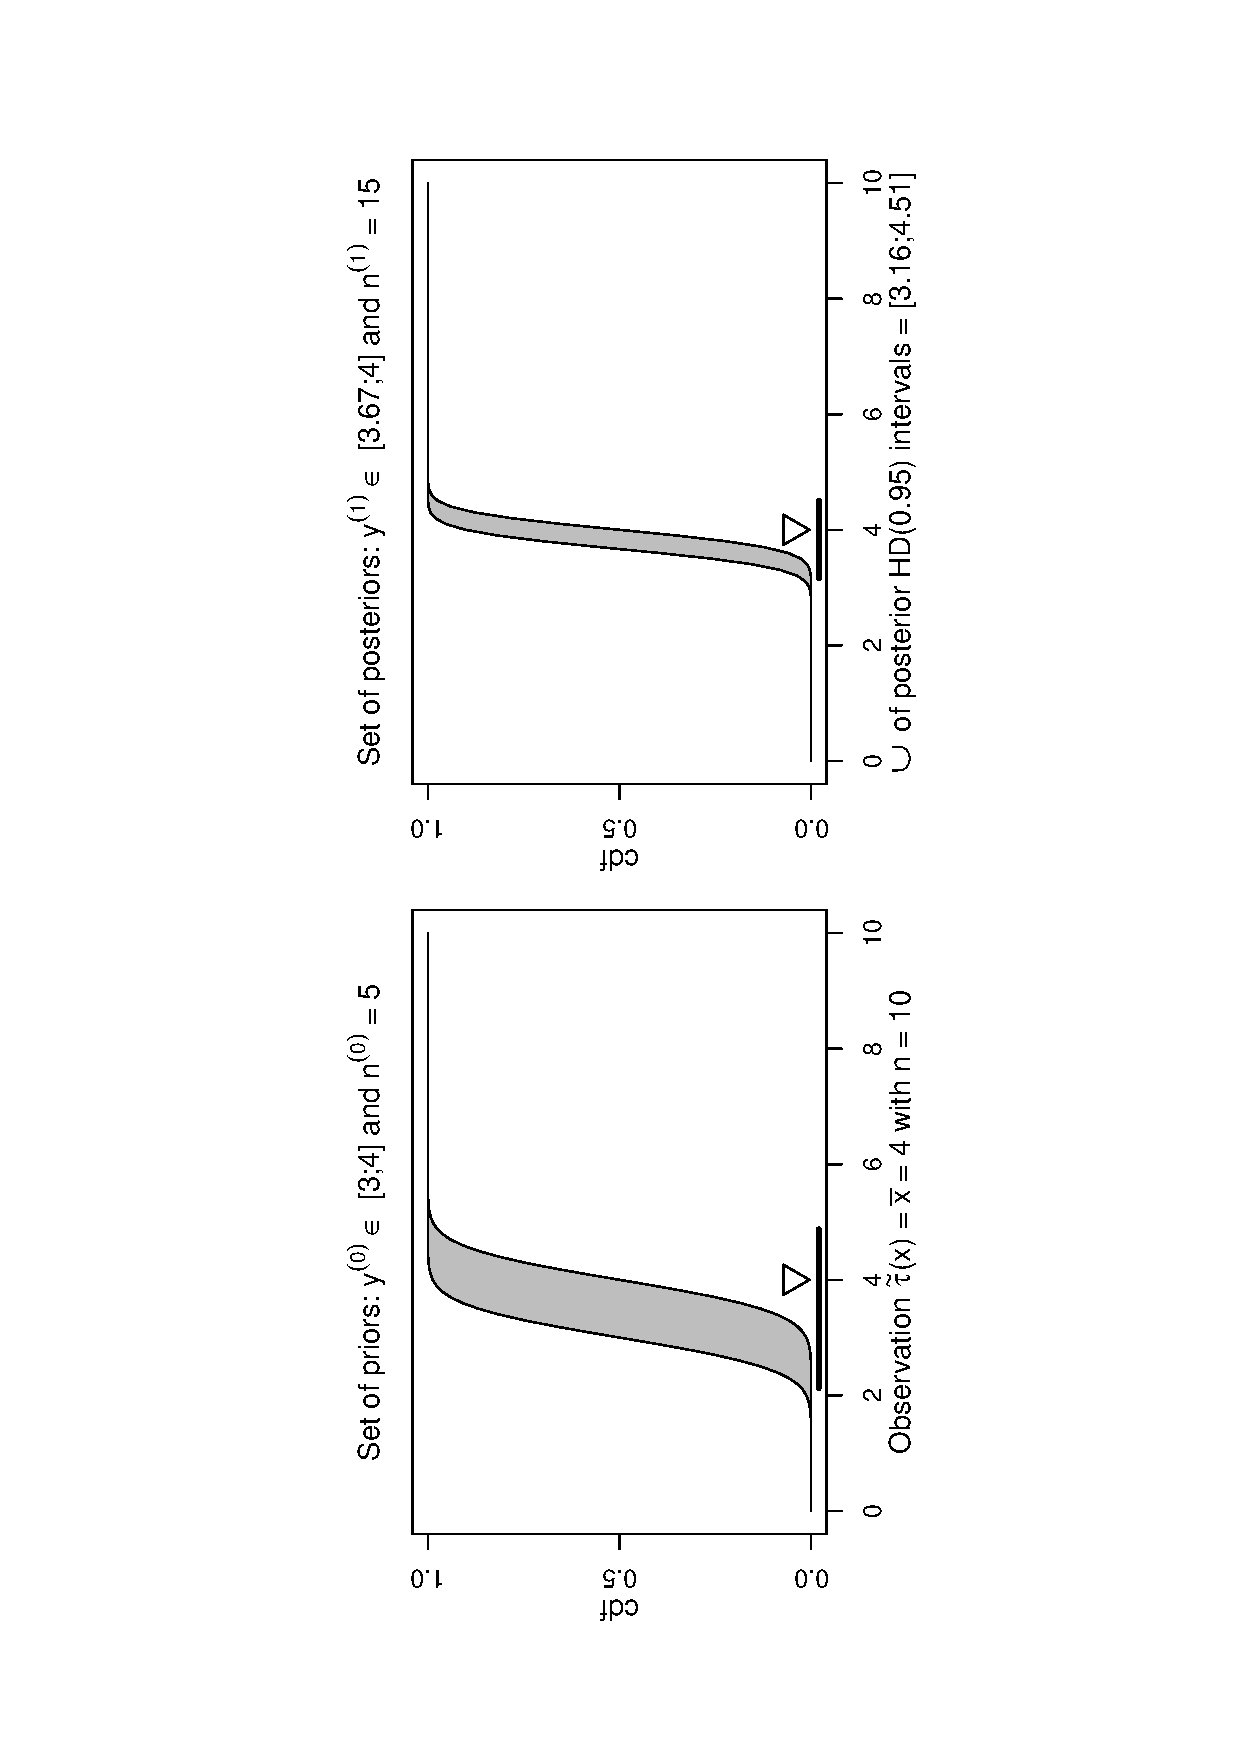
\includegraphics[trim = 20mm 50mm 20mm 50mm, clip, width=\textwidth]{fig/jstp-paper_nv_nfest_01-080331}%
\caption{Prior (left) and posterior (right) credal sets for a sample
from $\norm(\mu,1)$ drawn as sets of normal cdfs. (Example~\ref{ex:ymodel-nv} in the
situation of no prior data conflict.)}
\label{fig:nv-nfest-nopdc}
\end{figure}


\begin{example}[Normal-Normal Model]
\label{ex:ymodel-nv}
%\noindent\textbf{Example 1a (continued).}
In the Normal-Normal model as presented in Section~\ref{sec:norm-norm},
$\yz$ corresponds to the expected value for $\mu$; the choice of $\YZ$ in application should thus be easy.
To simplify notation, we will assume here and later on that $\sigma^2_0 = 1$.
%Assuming the prior knowledge suggests values for $\mu$ in the range $[3;4]$, we define
%${\cal Y}\uz = [\ul{y}\uz ; \ol{y}\uz] = [3;4]$. For fixing
Let us assume $\YZ = [\yzl ; \yzu] = [3;4]$, and for fixing
$\nz$, suppose further that we are not very certain about
this prior range for $\mu$, but still think it is quite a reasonable
assumption, and so we base it on $5$ pseudo observations by choosing $\nz=5$,
giving a value of the variance for the prior distribution on $\mu$ of $\frac{1}{5}$.
%
%\medskip
%
Updating this prior with the i.i.d.\ sample $\x \in \reals^n$ yields%\vspace*{-0.8ex}%
\begin{align*} %\label{080306-nv_bsp_held}
\ynl &= \frac{\nz\yzl + \sum_{i=1}^n x_i}{\nz + n}, &%\hspace*{-1.5ex}
\ynu &= \frac{\nz\yzu + \sum_{i=1}^n x_i}{\nz + n}, &%\hspace*{-1.5ex}
\nn &= \nz + n\,.%\vspace*{-3.1ex}%
\end{align*}

To make this concrete, consider a sample of size $n = 10$
with $\ttau(\x) = \bar{x} = 4$.
Then $\YN = [\frac{55}{15} ; \frac{60}{15}] \approx [3.67 ; 4]$,
${\rm MPI}\un=\frac{1}{3}$ and $\nn = 15$. The posterior credal set
consists therefore of all convex combinations of normal
distributions with means in $[3.67 ; 4]$ and variance
$\frac{1}{15}$.
%
% ------------ verschoben anfang
%
Prior and posterior beliefs can be illustrated by the union of
credal intervals calculated as highest density (HD) intervals%
\footnote{See the concept of highest posterior density (HPD) intervals
as mentioned in Section~\ref{sec:beta-binom}, which used here also to
illustrate the prior state of knowledge.}
%HD intervals\footnote{For a given distribution, a HD interval
%(for \emph{h}ighest \emph{d}ensity) gives a set
%of most plausible values identified as the set %with the shortest range
%of values with highest density
%resulting / aggregating a certain amount of probability weight $\gamma$.}
for all distributions in the corresponding credal set.
As the normal distributions with mean $\yz \in \YZ$ are the extreme points of the prior credal set,
and the normal distributions are stochastically ordered with respect to the mean,
the prior union is the interval from the lowest lower border of HD intervals
(calculated from $\norm(\yzl, \frac{1}{\nz})$) to the highest upper border
(calculated from $\norm(\yzu, \frac{1}{\nz})$).
For a probability weight $\gamma = 0.95$, we get $[2.123;\, 4.877]$.
%
% ------------ verschoben ende
%
The posterior union of HD intervals is
$[3.161;\, 4.506]$ and, covering a much smaller range as a priori, shows
the decreasing of uncertainty obtained by the update step, also
reflected in a main parameter precision gain of ${\rm PG}=\frac{2}{3}$.
This update step is illustrated in Figure~\ref{fig:nv-nfest-nopdc},
where the prior and posterior credal set are displayed by the normal
cumulative distribution functions, the black lines indicating the
functions defined by the vertices of $\YZ$ and $\YN$, respectively. %\sidenote{statt: that constitute their vertices.}
The observation $\ttau(\x)$ is marked by the point of the triangle
in both graphs, and the prior and posterior union of HD intervals are marked
by a thick line in the graph for the prior and posterior set, respectively.
\end{example}

\begin{example}[Dirichlet-Multinomial Model]
\label{ex:ymodel-idm}
An \ymodel\ based on the Dirichlet-Multinomial Model as discussed in Section~\ref{sec:diri-multi}
is, for $\YZ = \Y$, equivalent to the imprecise Dirichlet model
(IDM, see Section~\ref{sec:idm-and-near-ignorance}), and was considered in Section~\ref{sec:fixedlearningparameter}
for the common-cause failure application.

In the usual applications of the IDM, the aim is to start with prior
ignorance; this is modelled by choosing $\YZ$ as the unit
simplex. For $\nz$ values of 1 or 2 are suggested. Here,
we must rely on the interpretation of $\nz$ as prior strength, as
there is no interpretation in terms of other
parameters as in Example~1a.
%
%\medskip
%
Considering prior knowledge for a three-category multinomial model
suggesting that extreme values for $\theta_1$ and $\theta_2$ are
implausible, one could choose
$\YZ = \{ \yz_1 \in [0.2;0.8] \times \yz_2 \in [0.2;0.8] \times \yz_3 \in [0;0.6]\}$,
where the upper bound for $\yz_3$ is a result of the unit
simplex constraint $\sum_{j=1}^k \yz_j = 1$.
In addition, we choose again $\nz=5$ as in Example~\ref{ex:ymodel-nv}.
%
%\medskip
%
Considering a sample of size $5$, where $3$ observations are of
category 1, and $2$ of category 2, we get $\nn = 10$ and the ranges
$\yn_1 \in [0.4 ; 0.7]$,
$\yn_2 \in [0.3 ; 0.6]$, and
$\yn_3 \in [0   ; 0.3]$
for the posterior class probabilities.
%For instance, the posterior
%probability for observing category two or three in the next draw
%is, by applying conjugacy, between $0.3$ and $0.6$.
In analogy to Example~\ref{ex:ymodel-nv}, this update step is illustrated with the
left and center graph of Figure~\ref{fig:idm-nfest-nopdc}, where
prior and posterior credal sets are represented by cutouts from a
plane in the three-dimensional parameter space. Each point in the
plane cutout for the prior set on the left graph represents a
certain combination of $\yz_1$, $\yz_2$, and $\yz_3$ by the
magnitude of coordinates. The same applies for the posterior set
depicted in the center graph. Some additional lines were drawn to
make locating the cutouts in space more easy.
\end{example}

\begin{figure}
\begin{tabular}{ccc}%
\hspace*{-1.2ex}% trim = l b r t
%\includegraphics[height=0.33\textwidth,angle=-90,bb = 100 65 520 385]{fig/jstp-paper_idm_nfest_01-080331.ps}%
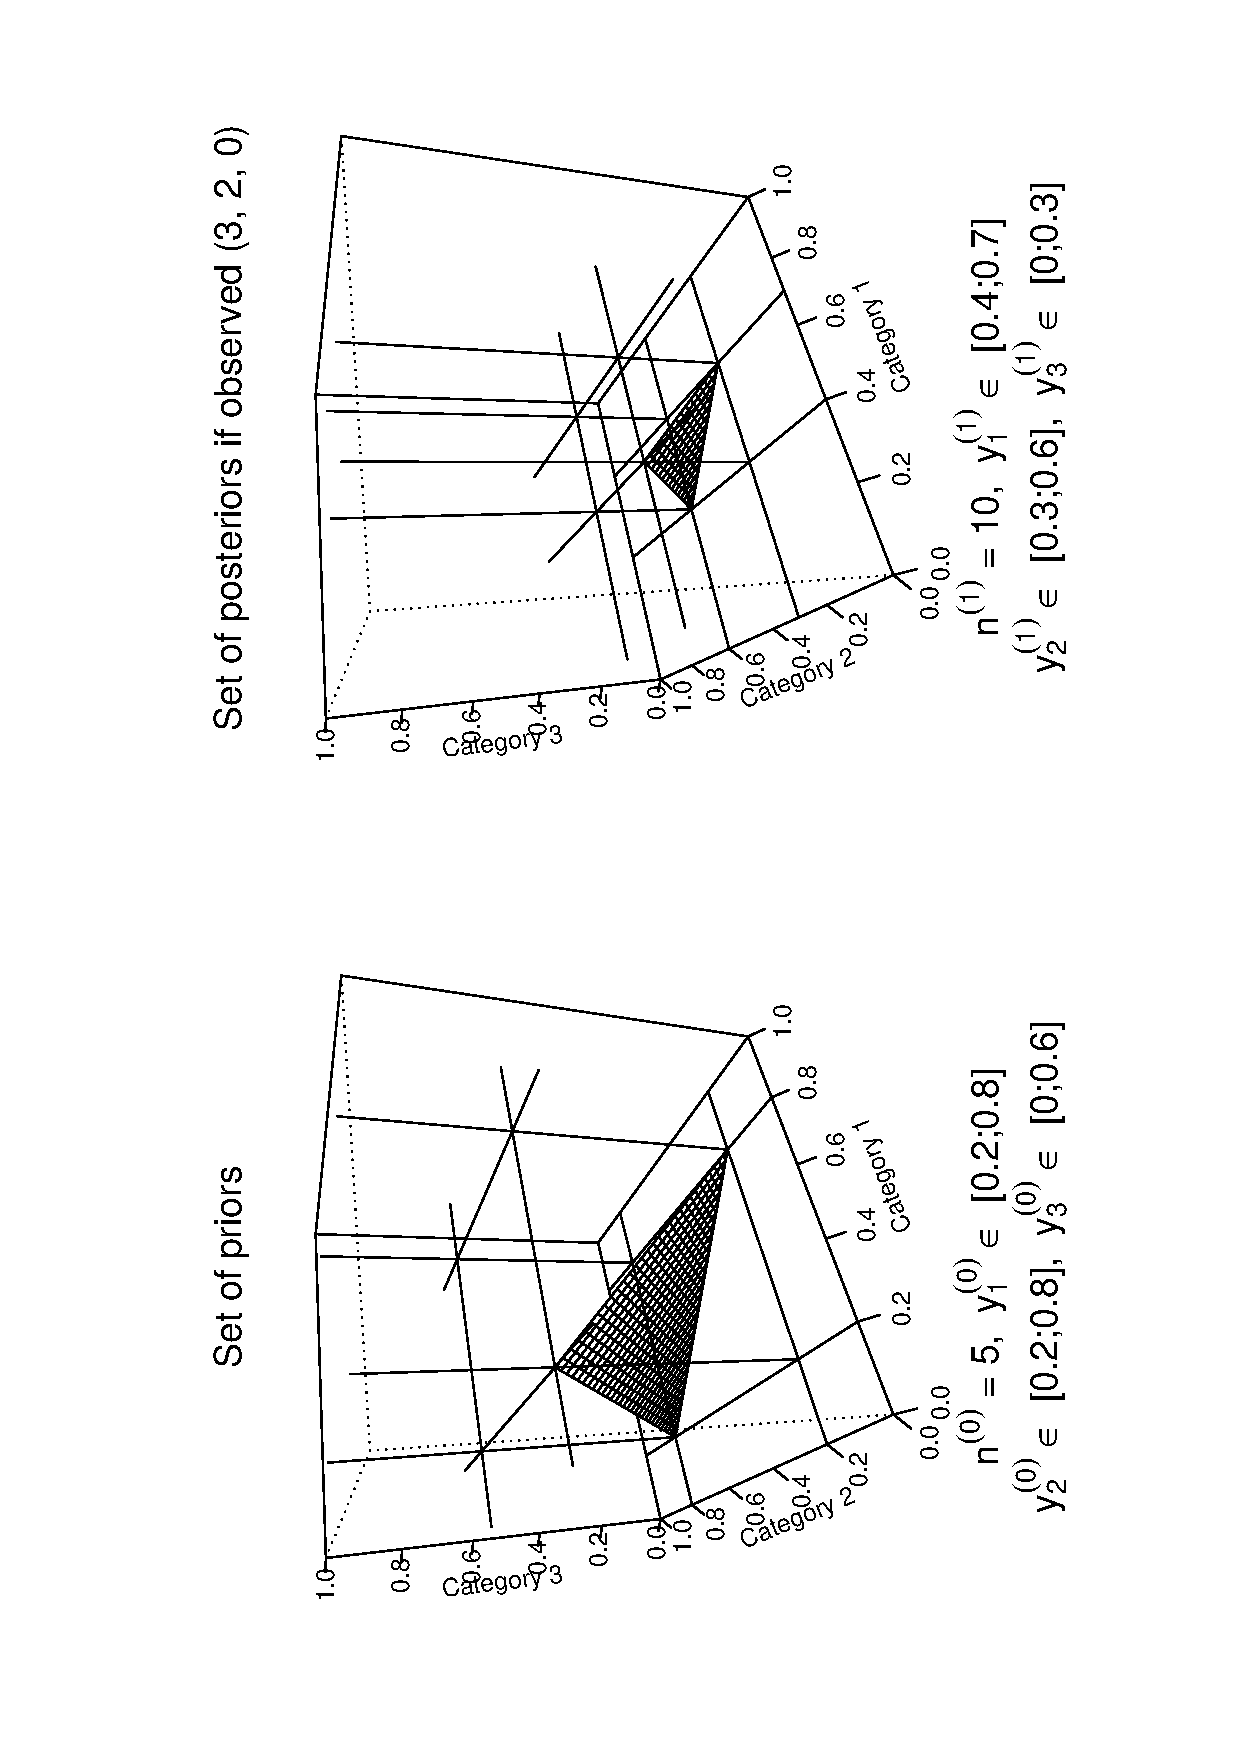
\includegraphics[trim =  20mm 25mm 150mm 20mm, clip, width=0.33\textwidth]{fig/jstp-paper_idm_nfest_01-080331}%
\hspace*{-1.2ex}%
&%
\hspace*{-1.2ex}%
%\includegraphics[height=0.33\textwidth,angle=-90,bb = 100 470 520 790]{fig/jstp-paper_idm_nfest_01-080331.ps}%
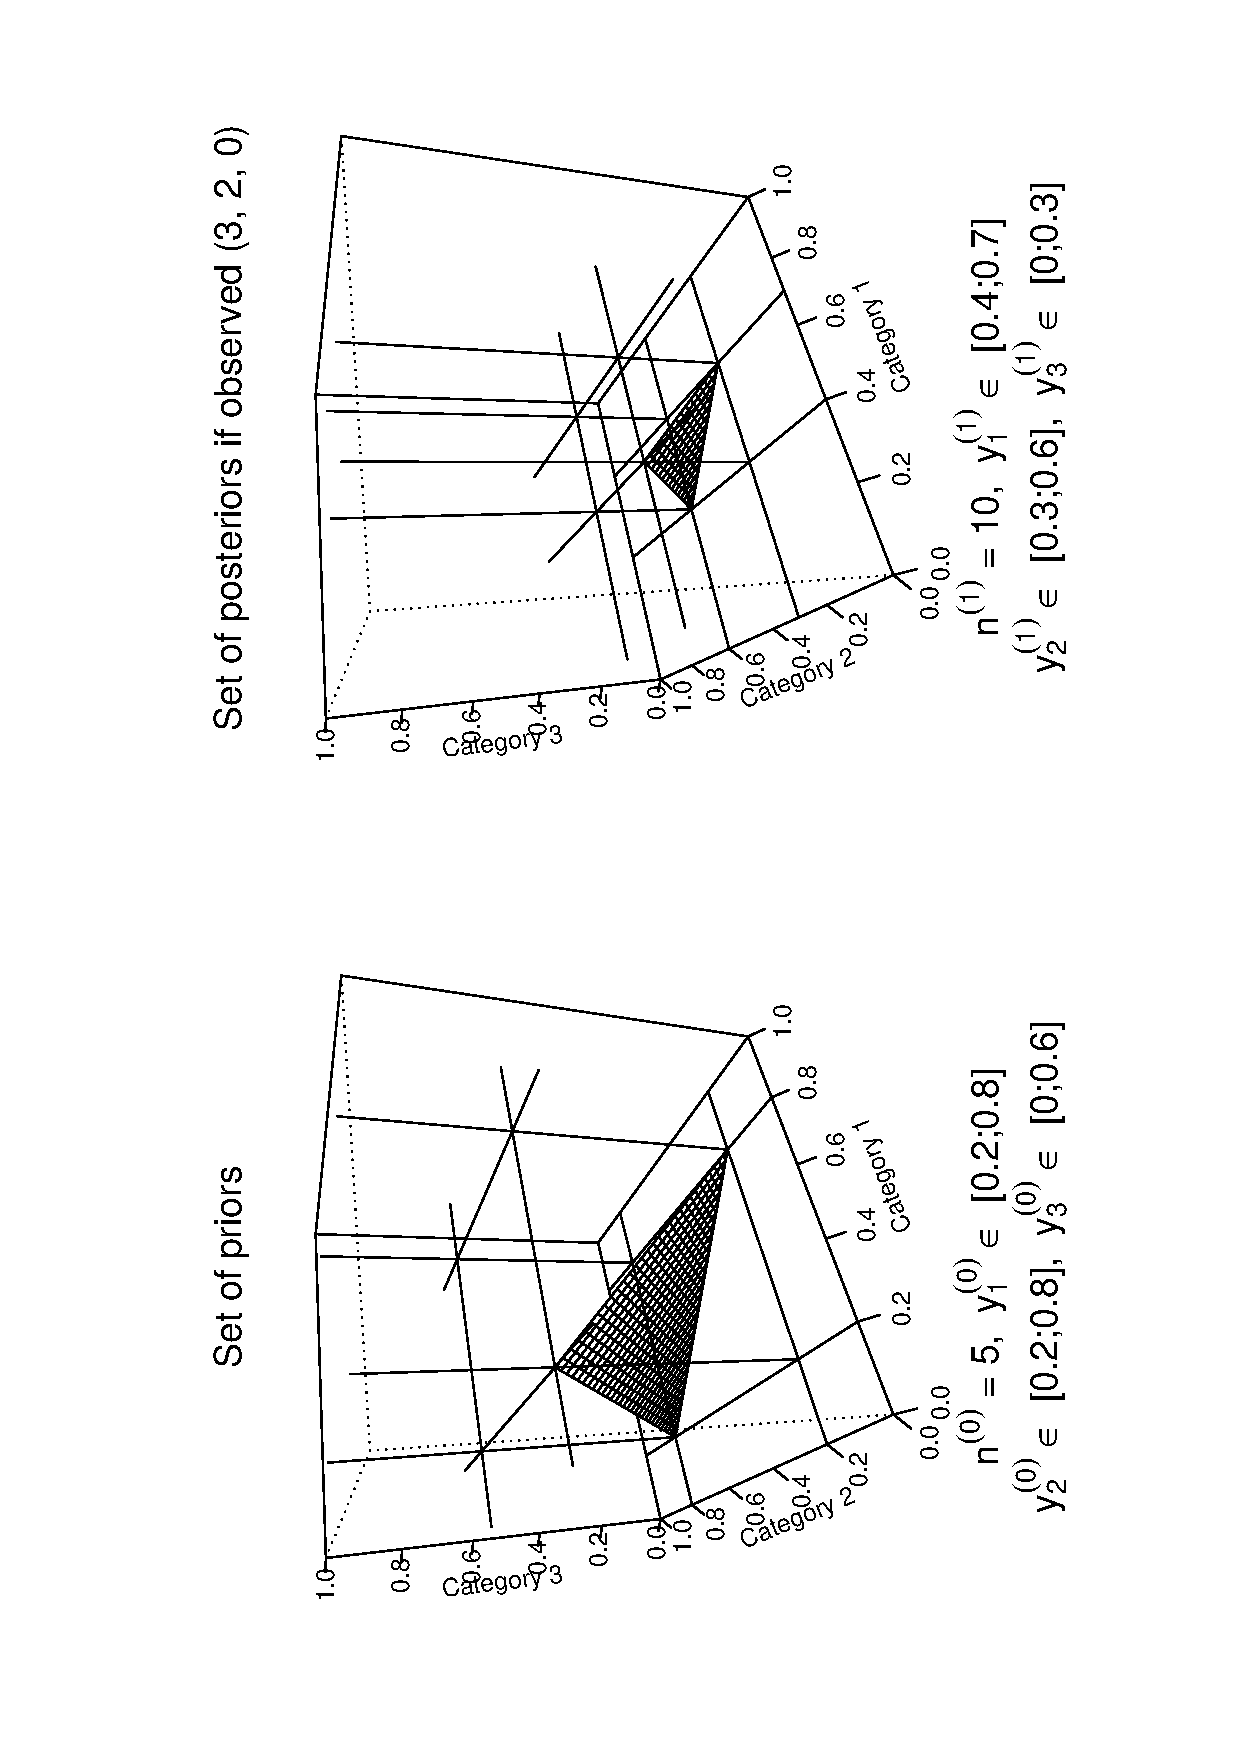
\includegraphics[trim = 150mm 25mm  20mm 20mm, clip, width=0.33\textwidth]{fig/jstp-paper_idm_nfest_01-080331}%
\hspace*{-1.2ex}%
&%
\hspace*{-1.2ex}%
%\includegraphics[height=0.33\textwidth,angle=-90,bb = 100 470 520 790]{fig/jstp-paper_idm_nfest_02-080331.ps}%
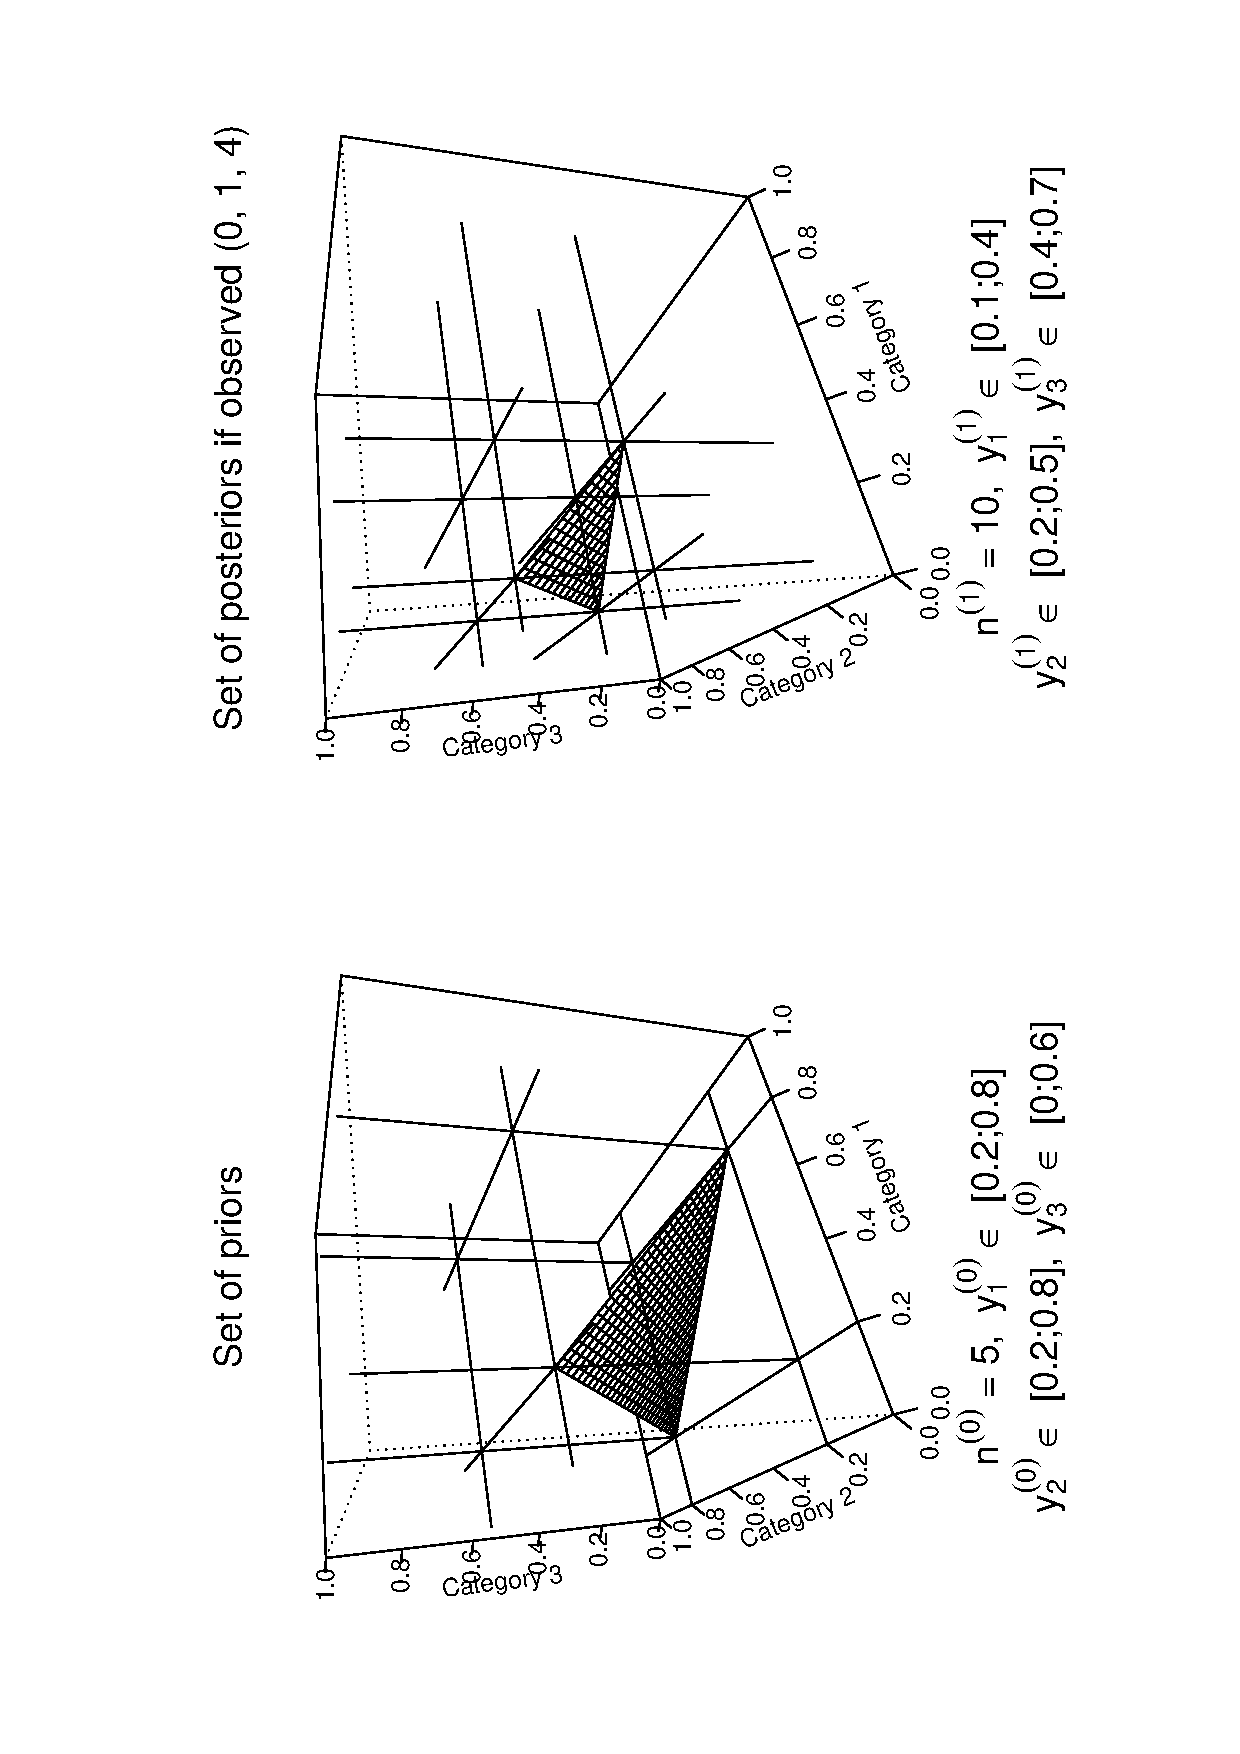
\includegraphics[trim = 150mm 25mm  20mm 20mm, clip, width=0.33\textwidth]{fig/jstp-paper_idm_nfest_02-080331}%
\hspace*{-1.2ex}%
\end{tabular}%
\caption{Prior (left) and posterior (center, right) credal sets for samples from
$\mult(\btheta)$ in accordance with (center) and, as studied in
Section~\ref{section:fixednschlecht}, contrary to (right) prior
beliefs. Note that both posterior sets have the same shape and size and differ
only in location, in contrast to the ones depicted in Figure~\ref{fig:idm-nvar-nopdc}.}
\label{fig:idm-nfest-nopdc}
\end{figure}


\begin{remark} \label{remark:i-v}
%The following list contains important properties of
%inference in \emph{\ymodel s}, \thc{where the first three items} in
%essence \thcc{generalize results} that have been discussed in
%the literature for the IDM, where, as already said above, $n\uz$
%usually is denoted by $s$.\vspace*{-1.5ex}
Inference in \emph{\ymodel s} has the following important properties,
where the first three items in essence generalize results that have
been discussed in the literature for the IDM, where, as already said
above, $\nz$ usually is denoted by $s$.%
\footnote{See the discussion in Section~\ref{sec:gbicp-properties-criteria}.***}
\begin{enumerate}[i)]
\item The larger $\nz$ relative to $n$, the more weight is placed on
the prior knowledge expressed by $\YZ$, resulting in wider
posterior expectation intervals and larger ${\rm MPI}\un$.
\item For growing sample sizes $n$, the set $\YN$ will
converge towards a one-element set, as the weight of the `imprecise'
$\YZ$ decreases with respect to the `precise' sample
$\ttau(\x)$, ultimately resulting in an (almost)
precise posterior with ${\rm MPI}\un=0$ just as in
classical methods.
\item In particular, for $\nz = n$, the width of the posterior
expectation interval is half the width of the prior interval,
i.e., ${\rm MPI}\un = \frac{1}{2}{\rm MPI}\uz$.
This property is easily derived from \eqref{equ:ymodel-ydiff}
below, and provides another vivid interpretation of $\nz$.
\item Ceteris paribus, a smaller choice of $\YZ$ will result
in a smaller $\YN$, leading to more precise inference
statements as opposed to the choice of a larger $\YZ$.%
\footnote{This item has not been widely considered in
the context of the IDM, which typically is used to
describe inference from a state of prior ignorance.}
\item For the main posterior parameter imprecision, we obtain:
\begin{align}\label{equ:ymodel-ydiff}
{\rm MPI}\un &= \frac{\nz \left( \yzu - \yzl \right)}{\nz + n}.
\end{align}
\end{enumerate}
\end{remark}%\vspace*{-1.5ex}
While items i) -- iv) demonstrate the intuitively appealing
behavior of \ymodel s, we are seriously concerned with %respect to
the fact that ${\rm MPI}\un$ is independent of $\ttau(\x)$,
and, as studied in more detail in the next subsection, therefore
insensitive to prior-data conflict.


\subsubsection{\ymodel s and Prior-Data Conflict}
\label{section:fixednschlecht}
In the linear setting of \ymodel s, the generic concept of prior-data conflict
can be formalized by considering the distance of the observed quantity $\ttau(\x)$ to
its nearest prior guess $\yz \in \YZ$:
%
\begin{definition}[(Degree of) Prior-Data Conflict]\label{080307-defin-pdc}
For \ymodel s, the degree of prior-data conflict can be defined %naturally
as
\begin{equation}\label{se-071217}
%\Delta \left(\frac{\tau^n(x)}{n};\, \ul{y}\uz,\,\ol{y}\uz\right)
%= \inf \left\{ \left| \frac{\tau^n(x)}{n} - y\uz \right|: \ul{y}\uz \leq y\uz \leq \ol{y}\uz \right\}\,.
\Delta \left(\ttau(\x);\, \yzl,\,\yzu\right)
:= \inf \left\{ \left| \ttau(\x) - \yz \right|: \yzl \le \yz \le \yzu \right\}\,.
\end{equation}
Consequently, if
$\Delta \left(\ttau(\x);\, \yzl,\,\yzu\right) > 0$,
we have an instance of prior-data conflict.%
\footnote{Instead of $\Delta(\;\;) > 0$, one could also consider some
threshold $\Delta(\;\;) > \varepsilon > 0$ as a criterion for prior-data conflict, making
Definition~\ref{080307-defin-pdc} also reasonable for \model s.
However, with respect to Remark~\ref{remark8} below, we prefer $\varepsilon = 0$.}
\end{definition}
This Definition can be illustrated by, e.g., Example~\ref{ex:ymodel-nv}, where $\ttau(\x) = \bar{x}$
is the sample mean. A sample mean outside $\YZ$, the a priori assumed interval
of means for the normal distribution on $\mu$, is an instance of prior-data conflict.
If a sample mean of $8$ was observed in the numerical example discussed above, where
$[\yzl ; \yzu] =[3;4]$ had been assumed, we would obtain $\Delta(\;) = 4$,
formalizing our intuition that prior-data conflict is at hand.

As we argued in Sections~\ref{sec:motivation:pdc} and **intro-here**,
imprecise probability models that allow to take prior information into account
should lead to more imprecision if prior-data
conflict is present than in situations where it is not.
%
It is easy to see that \ymodel s do not fulfill this property
because the main parameter posterior imprecision in
\eqref{equ:ymodel-ydiff} does not depend on the sample statistic
$\ttau(\x)$. Thus, for any sample of size $n$, an \ymodel\ leads
to the same main parameter posterior precision gain
whether the sample supports the prior assumptions modelled in
$\YZ$ or it confronts them. As a consequence of the
Bayesian paradigm that all inference is only allowed to depend on
the posterior, this holds also for all derived quantities
like HD intervals. To make this concrete,
let us continue Examples~\ref{ex:ymodel-nv} and \ref{ex:ymodel-idm}.

\begin{figure}
%\includegraphics[height=\textwidth,angle=-90,bb = 165 60 440 765]{fig/jstp-paper_nv_nfest_02-080331.ps}%
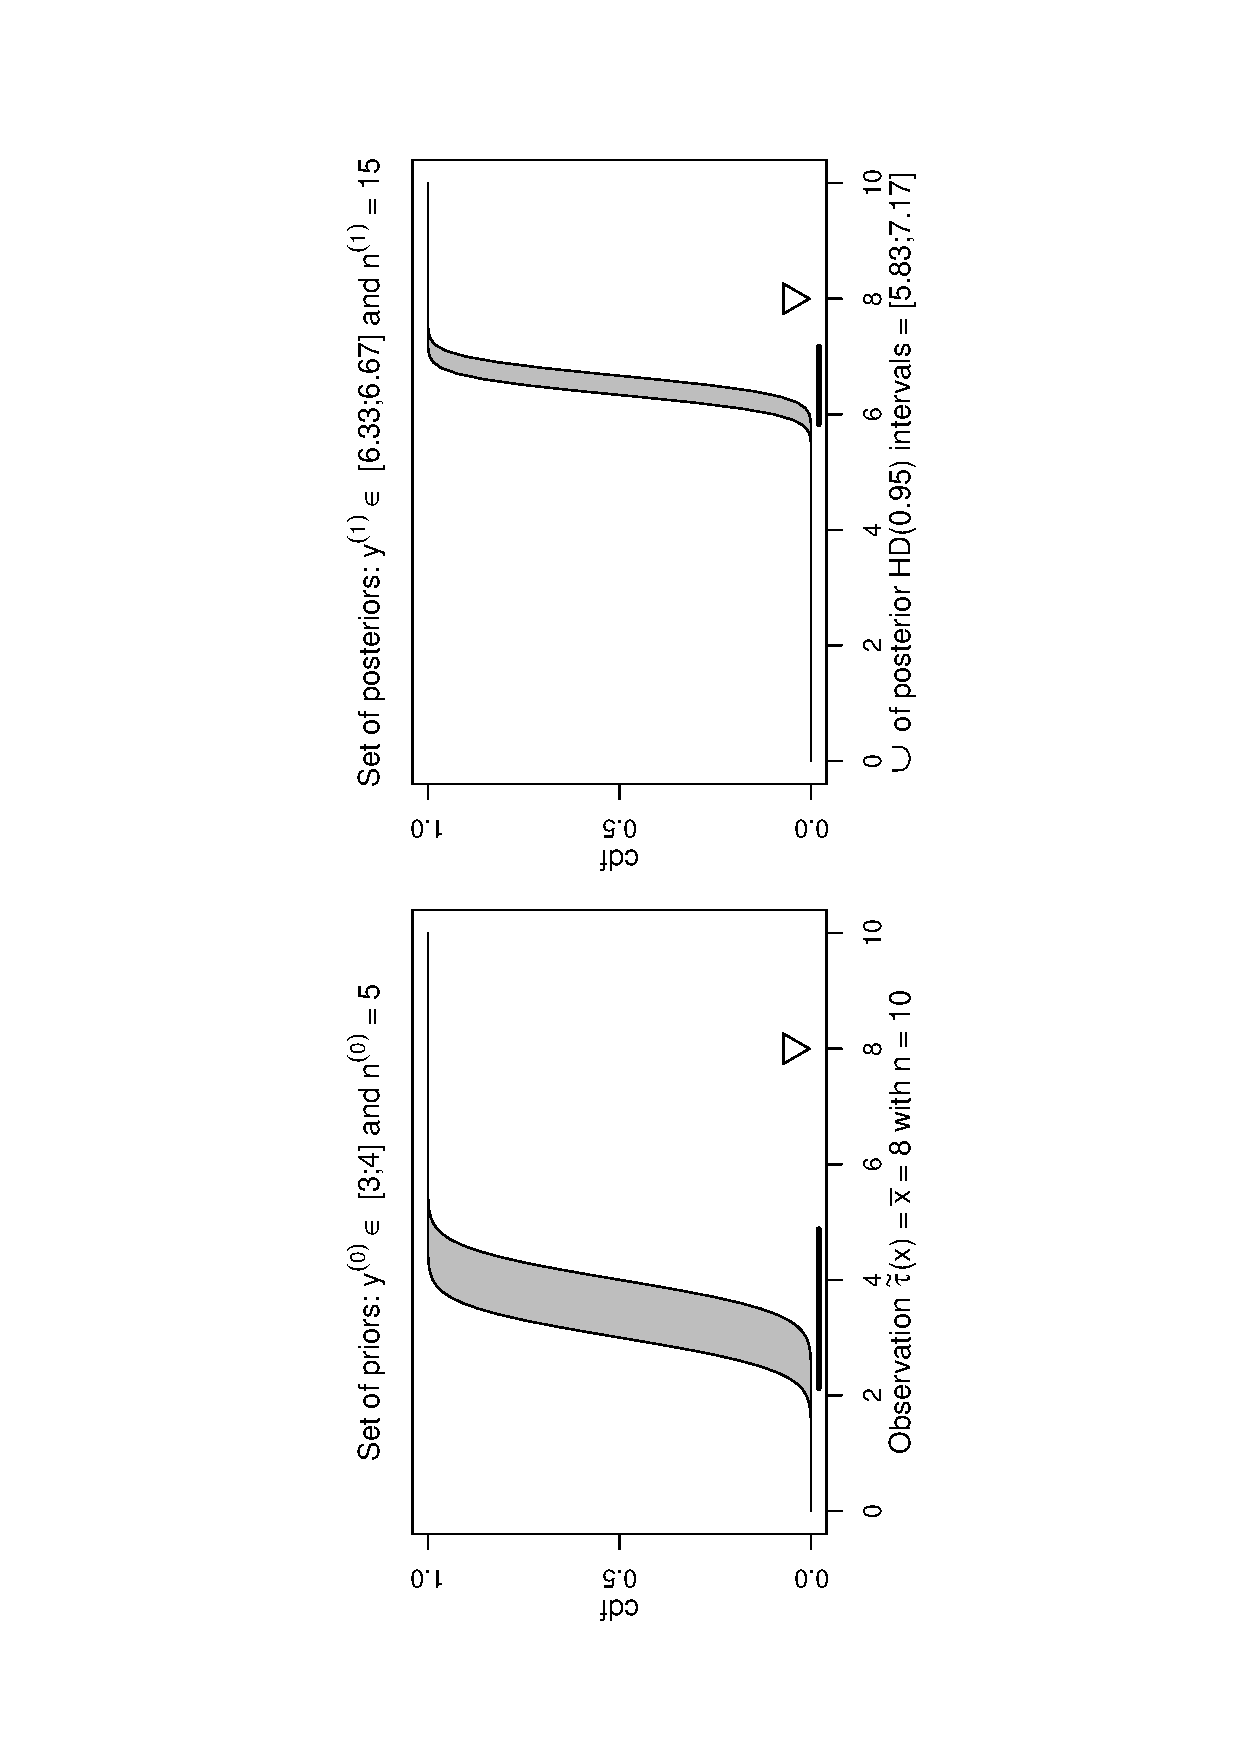
\includegraphics[trim = 20mm 50mm 20mm 50mm, clip, width=\textwidth]{fig/jstp-paper_nv_nfest_02-080331}%
\caption{In \ymodel s, an observation contrary to prior beliefs leads to
the same amount of imprecision as an observation in accordance with prior
beliefs (see Figure~\ref{fig:nv-nfest-nopdc}).  Generalized \ymodel s overcome this
deficiency, as visualized in Figure~\ref{fig:nv-nvar-vertfu}.}
\label{fig:nv-nfest-pdc}
\end{figure}

\begin{example}[Normal-Normal Model, continued]
\label{ex:jstp-5}
%\noindent\textbf{Example 1a (continued).}
Assume, in the situation considered in Section~\ref{070514-secImpPriorLUCK-QdC},
that the sample had led to $\ttau(\x) = 8$,
suggesting the mean $\mu$ to be nearer to $8$ than to the range $[3;4]$ assumed
for it before having seen the sample.
Then $\YN = [\frac{95}{15} ; \frac{100}{15}] \approx [6.33 ; 6.67]$ and again
$\nn = 15$. The posterior range of expected values for $\mu$ has now moved
towards the value suggested by the sample, but we have the same
posterior main parameter imprecision $\frac{1}{3}$ as in the
case with $\ttau(\x) = 4$, which was not conflicting with the prior
assumptions. Intuitively, this fact gets maybe more perplexing when
considering the union of posterior HD intervals: For $\ttau(\x) = 4$,
it is $[3.161;\, 4.506]$, covering a length of $1.345$; for
$\ttau(\x) = 8$, it is $[5.827;\,7.172]$, covering the very same
length, and therefore -- although being completely surprised by the
outcome of the sample -- we would not be more cautious.
These disturbing results are illustrated in Figure~\ref{fig:nv-nfest-pdc}.
\end{example}

\begin{example}[Dirichlet-Multinomial Model, continued]
\label{ex:jstp-6}
%\noindent\textbf{Example 1b (continued).}
Here, the same phenomenon occurs:
Having observed categories 1 to 3 now $0$, $1$, and $4$
times, respectively, $\YN$ covers the same area, despite of the clear conflict of these
observations with the prior knowledge expressed in $\YZ$,
and has only moved in location, as can be seen
in the right graph of Figure~\ref{fig:idm-nfest-nopdc}.
\end{example}


\subsection{Improved imprecise priors for inference in \model s}
\label{sec:4-gw-071216}

There do exist some imprecise probability models that react on
prior-data conflict in reasonable ways. The approaches by
\textcite{1991:pericchi} and \textcite{1994:coolen}
are restricted to specific one-parameter situations with a different type
of models for the prior. \textcite{2005:whitcomb}, on
the other hand, by partially relying on models from the exponential
family, considers closely related classes of underlying
distributions without using their specific structure. The important
hint for properly handling prior-data conflict in
\model s is again obtained from \textcite{1991:walley}.
In \S 5.4, he discusses prior-data conflict in the imprecise
Beta-Binomial model,%
\footnote{See Section~\ref{sec:beta-binom}.}
which is a special case of the Imprecise
Dirichlet Model recalled in Example~\ref{ex:ymodel-idm}. His successful idea is to
vary the hyperparameter $s$ in addition. Additionally, he also
briefly mentions the normal case underlying Example~\ref{ex:ymodel-nv}
\parencite[\S 1.1.5 (k)]{1991:walley}, where he suggests to use an
imprecise prior with an imprecise variance. In the light of the
general framework of \model s, both exemplary solutions
can be subsumed under the idea to use an imprecise prior strength,
thus weighting prior and sample information in
\eqref{equ:shifttrans} in a more flexible way, i.e.\ to vary
additionally the prior strength parameter $\nz$ in some set $\NZ$.
Indeed this way to proceed will turn out to be successful.
We start by describing the powerful generalization we want to
propose in more detail and then discuss some of its basic
properties.
%
%
%
%
\begin{definition}[\nymodel s]\label{071221-def}%
%Consider the Imprecise Probability model as described in \mycite{QdC} %Quaeghebeur and de Cooman (2005),
%or, more generally, a \textsc{LUCK}-model,
Consider the situation of Definitions~\ref{070503-defin1}
and \ref{071219-def2}, and a set of LUCK-models
$\big(p(\vartheta),p(\vartheta\mid\x)\big)$ that is produced by
$\yz$ varying in some set $\YZ \subset \Y$
and, in addition, $\nz$ varying in a set $\NZ \subset \posreals$.
Let furthermore again the credal sets ${\cal M}$ and ${\cal M}_{|\x}$ consist
of all convex mixtures obtained from this variation of $p(\vartheta)$ and
$p(\vartheta\mid\x)$. Then $\big({\cal M}, {\cal M}_{|\x}\big)$ is
called the corresponding \emph{\nymodel } based on $\YZ$ and $\NZ$.
\end{definition}

\begin{remark}
Again, by construction, when ${\cal M}$ is used as an
imprecise prior,  ${\cal M}_{|\x}$ is the corresponding posterior. It is obtained
as the set of all convex mixtures of
distributions defined by the parameter set
\begin{equation*}
%\left\{\!\! \left. \left(\!n\uo,\, y\uo\! \right) \; \right| \; n\uo = n\uz + n,\, y\uo = \frac{n\uz y\uz + \tau(x)}{n\uz+n},\,
%n\uz \in {\cal N}\uz,\, y\uz \in {\cal Y}\uz \!\right\}
\left\{ \left. \left(\nn,\yn\right) \; \right| \, \nn = \nz + n,\, \yn = \frac{\nz\yz + \tau(\x)}{\nz + n},\,
\nz \in \NZ,\, \yz \in \YZ \right\}\,.
\end{equation*}
Note that the set of posterior parameters is not a cartesian product, i.e., rectangular. However,
extreme values for the main posterior parameter $\yn$ are still easy to derive:%
\footnote{As $\frac{d}{d \yz}\, \yn = \frac{\nz}{\nz + n} \ge 0 \;
\forall\, n,\, \nz,\,\tau(\x)$, it holds that $\yn$ is growing in
$\yz$ regardless of the value of $\nz$, and thus, for obtaining
$\ynu$, we must insert $\yzu$, and for obtaining
$\ynl$, we must insert $\yzl$ in \eqref{070305-4}, just as
in \ymodel s, where $\nz$ is fixed. Then, with
$\frac{d}{d \nz}\, \yn  = \frac{\yz n - \tau(\x)}{(\nz + n)^2}$, we see that $\yn$
is growing in $\nz$ if $\yz > \ttau(\x)$ and decreasing in
$\nz$ if $\yz < \ttau(\x)$, leading to
Equations~\eqref{equ:uly1-071206} and \eqref{equ:oly1-071206}.}

\begin{align}
\ynl &= \label{equ:uly1-071206}
\begin{cases}
\frac{\nzu \yzl + \,\tau(\x)}{\nzu + n} & \text{if}\quad \ttau(\x) \ge \yzl\\[1.5ex]
\frac{\nzl \yzl + \,\tau(\x)}{\nzl + n} & \text{if}\quad \ttau(\x) <   \yzl
\quad\Longleftrightarrow\quad \text{prior-data conflict}
\end{cases} \\[1ex]
\ynu &= \label{equ:oly1-071206}
\begin{cases}
\frac{\nzu \yzu + \,\tau(\x)}{\nzu + n} & \text{if}\quad \ttau(\x) \le \yzu\\[1.5ex]
\frac{\nzl \yzu + \,\tau(\x)}{\nzl + n} & \text{if}\quad \ttau(\x) >   \yzu
\quad\Longleftrightarrow\quad \text{prior-data conflict}.
\end{cases}
\end{align}
\end{remark}

For minimizing and maximizing $\yn$, the value $\nzl$ is
used only in the situation of prior-data conflict, that is, if
$\ttau(\x) \notin \YZ$.
When no prior-data conflict occurs, the extreme values are attained for $\nzu$.
%
Therefore, the fixed value of $\nz$ in \ymodel s in the spirit of \textcite{2005:quaeghebeurcooman} can be
seen as the upper border of an implicit set $\NZ$, and
considering only a fixed $\nz$ means that prior-data conflict is neglected.

On the other hand, if observations are such that
$\ttau(\x) \in \left[\yzl;\,\yzu\right]$, then
no prior-data conflict is present, and inference in \nymodel s
leads to very similar results as inference in \ymodel s.%
\footnote{From \eqref{equ:uly1-071206} and \eqref{equ:oly1-071206}
it gets clear why varying $\nz$ in addition does change the
update step in the desired way. When $\ttau(\x) < \yzl$,
then $\nzu$ is still used to calculate $\ynu$, but
$\nzl$ to calculate $\ynl$. The use of $\nzl$ instead
of $\nzu$ results in a lower value for $\yzl$, as then
more weight is given to $\ttau(\x)$ with respect to
$\yzl$. (Equation~\eqref{equ:shifttrans} makes this most
visible.) The same type of reasoning applies for the case
$\ttau(\x) > \yzu$, where $\nzu$ is still used to
calculate $\ynl$, but $\nzl$ to calculate $\ynu$.}

\begin{remark}\label{remark8}
By construction, the attractive properties of inferences by
\ymodel s formulated in i) to iv) of Remark~\ref{remark:i-v}
are still satisfied in our extended model. Now
also in addition prior-data conflict is handled in a
convincing way: Considering the relationship between the main
parameter posterior imprecision defined as in
\emph{\eqref{071214-4}} and the degree of prior-data conflict
as defined in \emph{\eqref{se-071217}},%
\footnote{Remark~\ref{071221-remark} and Definition~\ref{080307-defin-pdc} can directly be applied also to \nymodel s.}
the very same results as derived by \textcite[p.~224]{1991:walley}
for the two-category Dirichlet-Multinomial model hold in general
for any \nymodel: %\vspace*{-1.0ex}

%Using the update rules for varying $n\uz$, we get,
%just as described in Walley (1991, p.~224) for a two-category IDM,
%a posterior range of
%\vspace*{-3.0ex}
\begin{align*}
{\rm MPI}\un &= \frac{\nzu (\yzu - \yzl)}{\nzu + n}
                + \Delta \left(\ttau(\x);\, \yzl,\,\yzu\right)
                  \, \frac{n (\nzu - \nzl)}{(\nzu + n)(\nzl + n)}\,.%
\end{align*}
%\vspace*{-1.0ex}
It is only through $\Delta(\;)$ that ${\rm MPI}\un$ is 
depending on the actual shape of observation $\x$ besides its size
$n$, and increasing it if prior-data conflict occurs. When no
prior-data conflict is present, $\Delta \left(\ttau(\x);\,\yzl,\,\yzu\right) = 0$,
and we have the same amount of posterior imprecision in substantial parameters as in \emph{\ymodel s},
given by \emph{\eqref{equ:ymodel-ydiff}}.
%
Consequently, Walley's \parencite*[\S 5.4, footnote~3]{1991:walley} observation
that the factor to $\Delta(\;)$ gets maximal if $n = \big(\nzl\nzu\big){}^\frac{1}{2}$
remains valid. Then, the main parameter posterior imprecision
is maximal for a given degree of conflict, implicitly telling that
then the weight of the prior and sample must be the same, as more
weight on any of them compared to the other (preferring one source
of information to the other) would lead to a less wide $\YN$.
This fact gives additional orientation for choosing $\NZ$,
by considering the global strength of prior knowledge,
being equivalent to $\ul{\ol{n}}\uz := \big(\nzl\nzu\big){}^\frac{1}{2}$.
\end{remark}

\begin{figure}
%\includegraphics[height=\textwidth,angle=-90,bb = 90 60 515 770]{fig/jstp-paper_nv_nvar_vertfu01_081128.ps}%
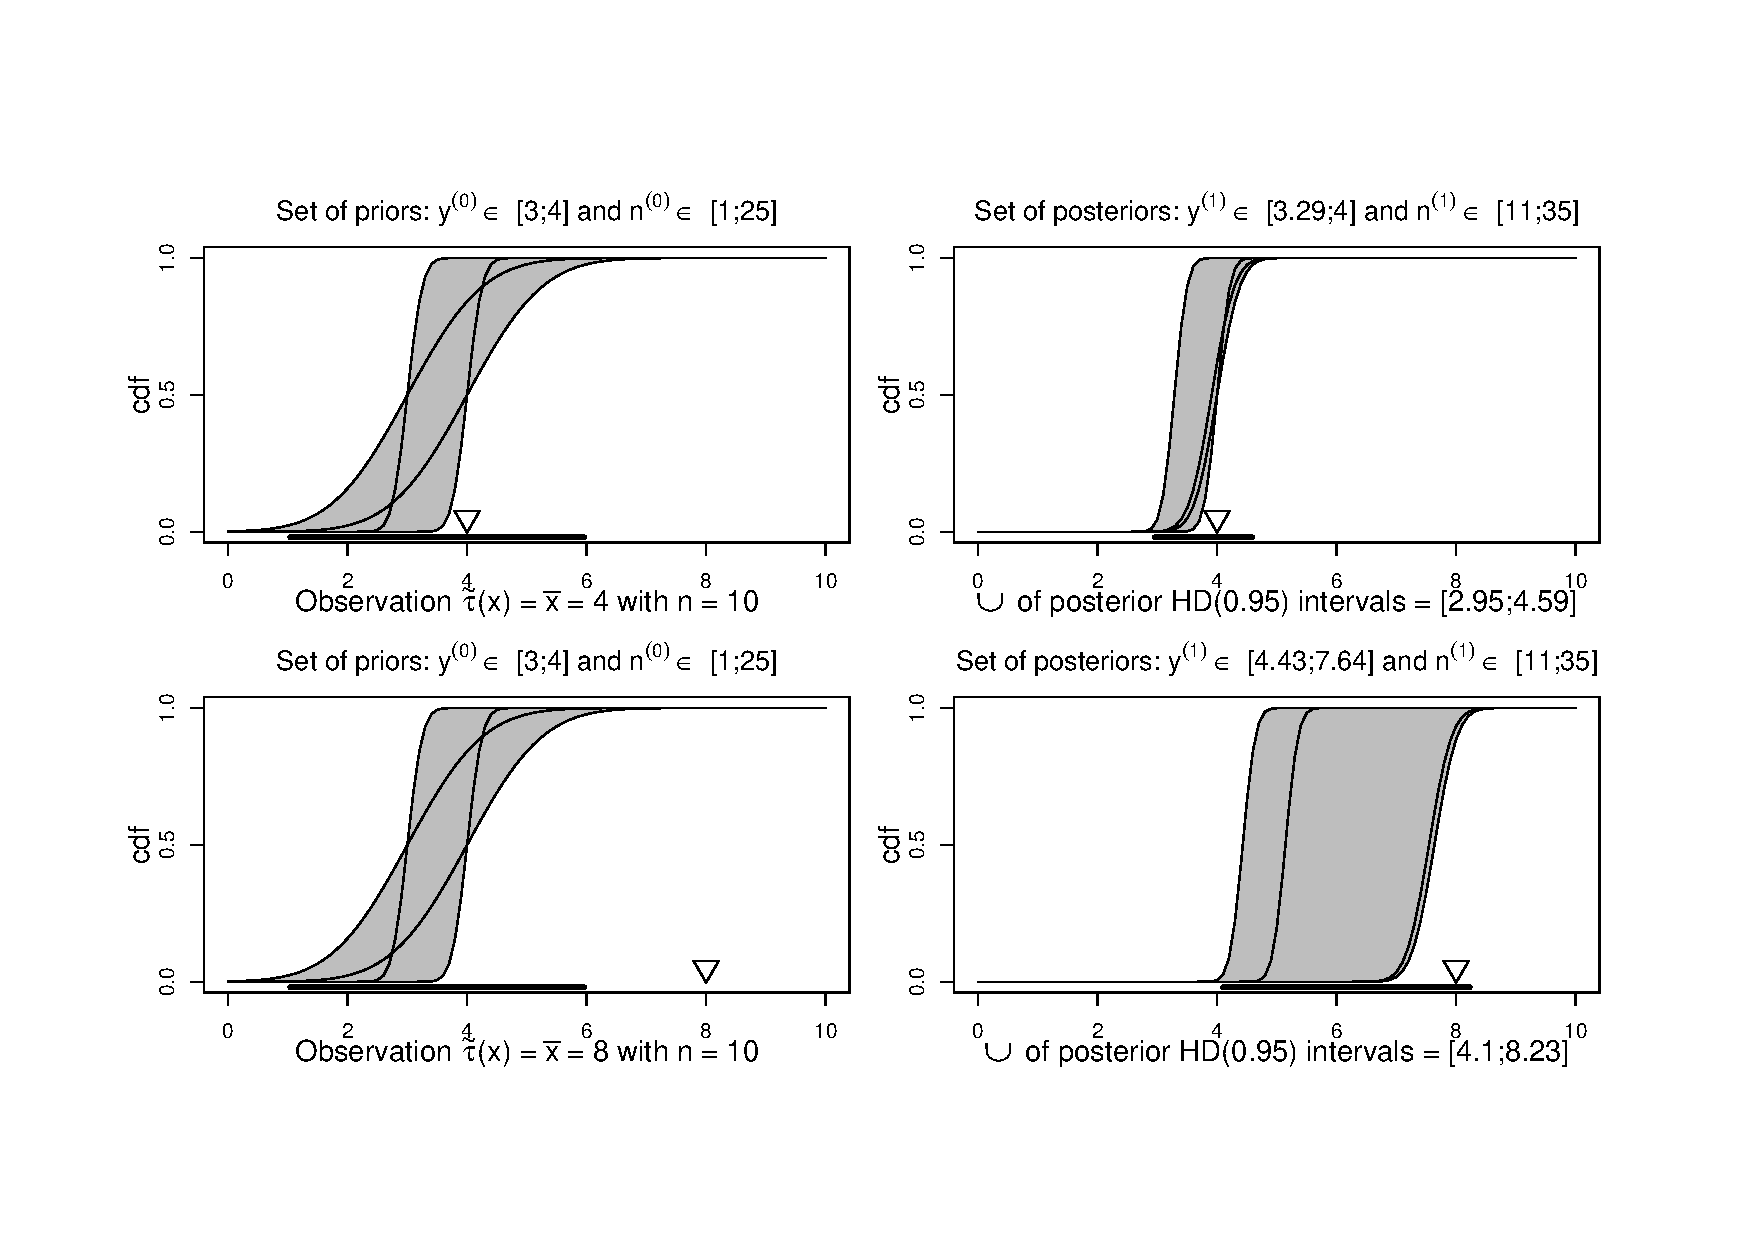
\includegraphics[trim = 20mm 20mm 20mm 25mm, clip, width=\textwidth]{fig/jstp-paper_nv_nvar_vertfu01_081128}%
\caption{Prior (left) and posterior (right) credal sets for samples from
$\norm(\mu,1)$ in accordance with (upper) and contrary to (lower)
prior beliefs. With \nymodel s, the posterior set in the latter case is
significantly larger than in the former, leading to more cautious inference as desired.}
\label{fig:nv-nvar-vertfu}
\end{figure}


\subsection{Illustration of the \nymodel} \label{sec:illu} 

The theoretical considerations in Section~\ref{sec:4-gw-071216} are now
illustrated by means of Examples~\ref{ex:ymodel-nv} -- \ref{ex:jstp-6},
and some simulated data for larger sample sizes.

\begin{example}[Normal-Normal model, continued]
\label{ex:jstp-7}
For the case of the Normal-Normal Model (Examples~\ref{ex:ymodel-nv} and \ref{ex:jstp-5}),
the behavior of an appropriate \nymodel\ is shown for the situations previously
modeled with an \ymodel\ as depicted in
Figures~\ref{fig:nv-nfest-nopdc} and \ref{fig:nv-nfest-pdc}. In
Figure~\ref{fig:nv-nvar-vertfu}, the top row shows the updating in
absence of prior-data conflict, whereas the lower row displays
the update step in presence of prior-data conflict.
Again, the vertices of the credal set, the set of normal
distribution functions, is represented by the shaded area,
and the lines indicate the distributions that are obtained by updating the four
extreme distributions from $\NZ \times \YZ$.

Contrary to the \ymodel, also a range of variances is considered in the
prior, allowing for reasonable posterior inference, as can be seen
in the right hand graphs: when the prior model is consistent with
the observation $\ttau(\x) = \bar{x}$, a similar union of posterior HD
intervals is obtained as for the model displayed in
Figure~\ref{fig:nv-nfest-nopdc}; when instead prior assumptions and
data are conflicting, the posterior credal set reflects our
uncertainty on which to trust, being substantially larger than the
prior credal set. Therefore, the union of posterior HD intervals as
indicated by the thick line in the lower right graph is not only
wider than in the absence of prior-data conflict as seen in the top
right graph, but not much shorter than its prior counterpart which is $[1.040;\, 5.960]$.
In order to give comparable results, $\NZ$ was chosen to give the same global prior strength as the
\ymodel\ for Example~\ref{ex:ymodel-nv} by fixing $\ul{\ol{n}}\uz=5$ and a minimal prior strength
$\nzl = 1$, resulting in $\nzu = 25$.
\end{example}

\begin{figure}
%\fbox{%
\begin{tabular}{ccc}%
\hspace*{-1.2ex}%
%\includegraphics[height=0.33\textwidth,angle=-90,bb = 100 65 520 385]{fig/jstp-paper_idm_nvar_zeile1-080331.ps}%
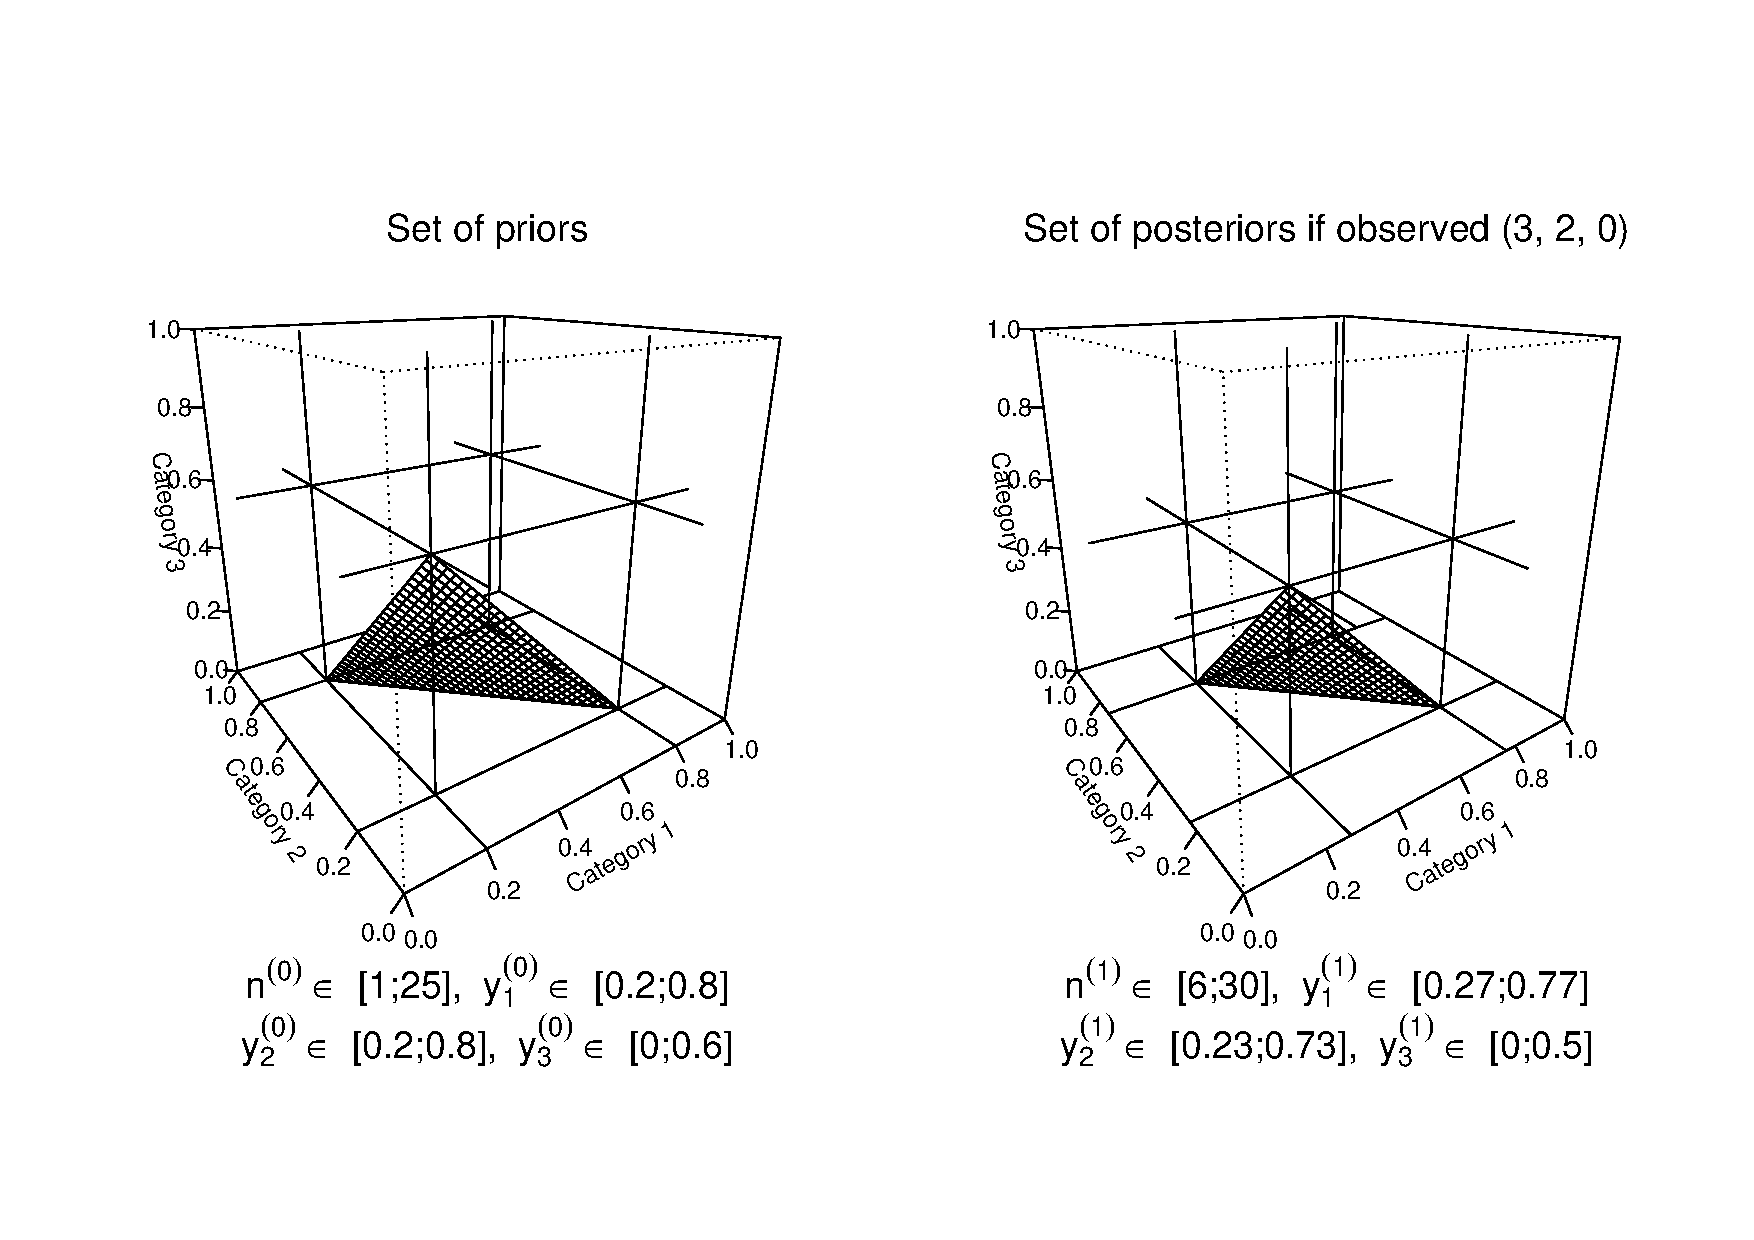
\includegraphics[trim =  20mm 25mm 150mm 20mm, clip, width=0.33\textwidth]{fig/jstp-paper_idm_nvar_zeile1-080331}%
\hspace*{-1.2ex}%
&%
\hspace*{-1.2ex}%
%\includegraphics[height=0.33\textwidth,angle=-90,bb = 100 470 520 790]{fig/jstp-paper_idm_nvar_zeile1-080331.ps}%
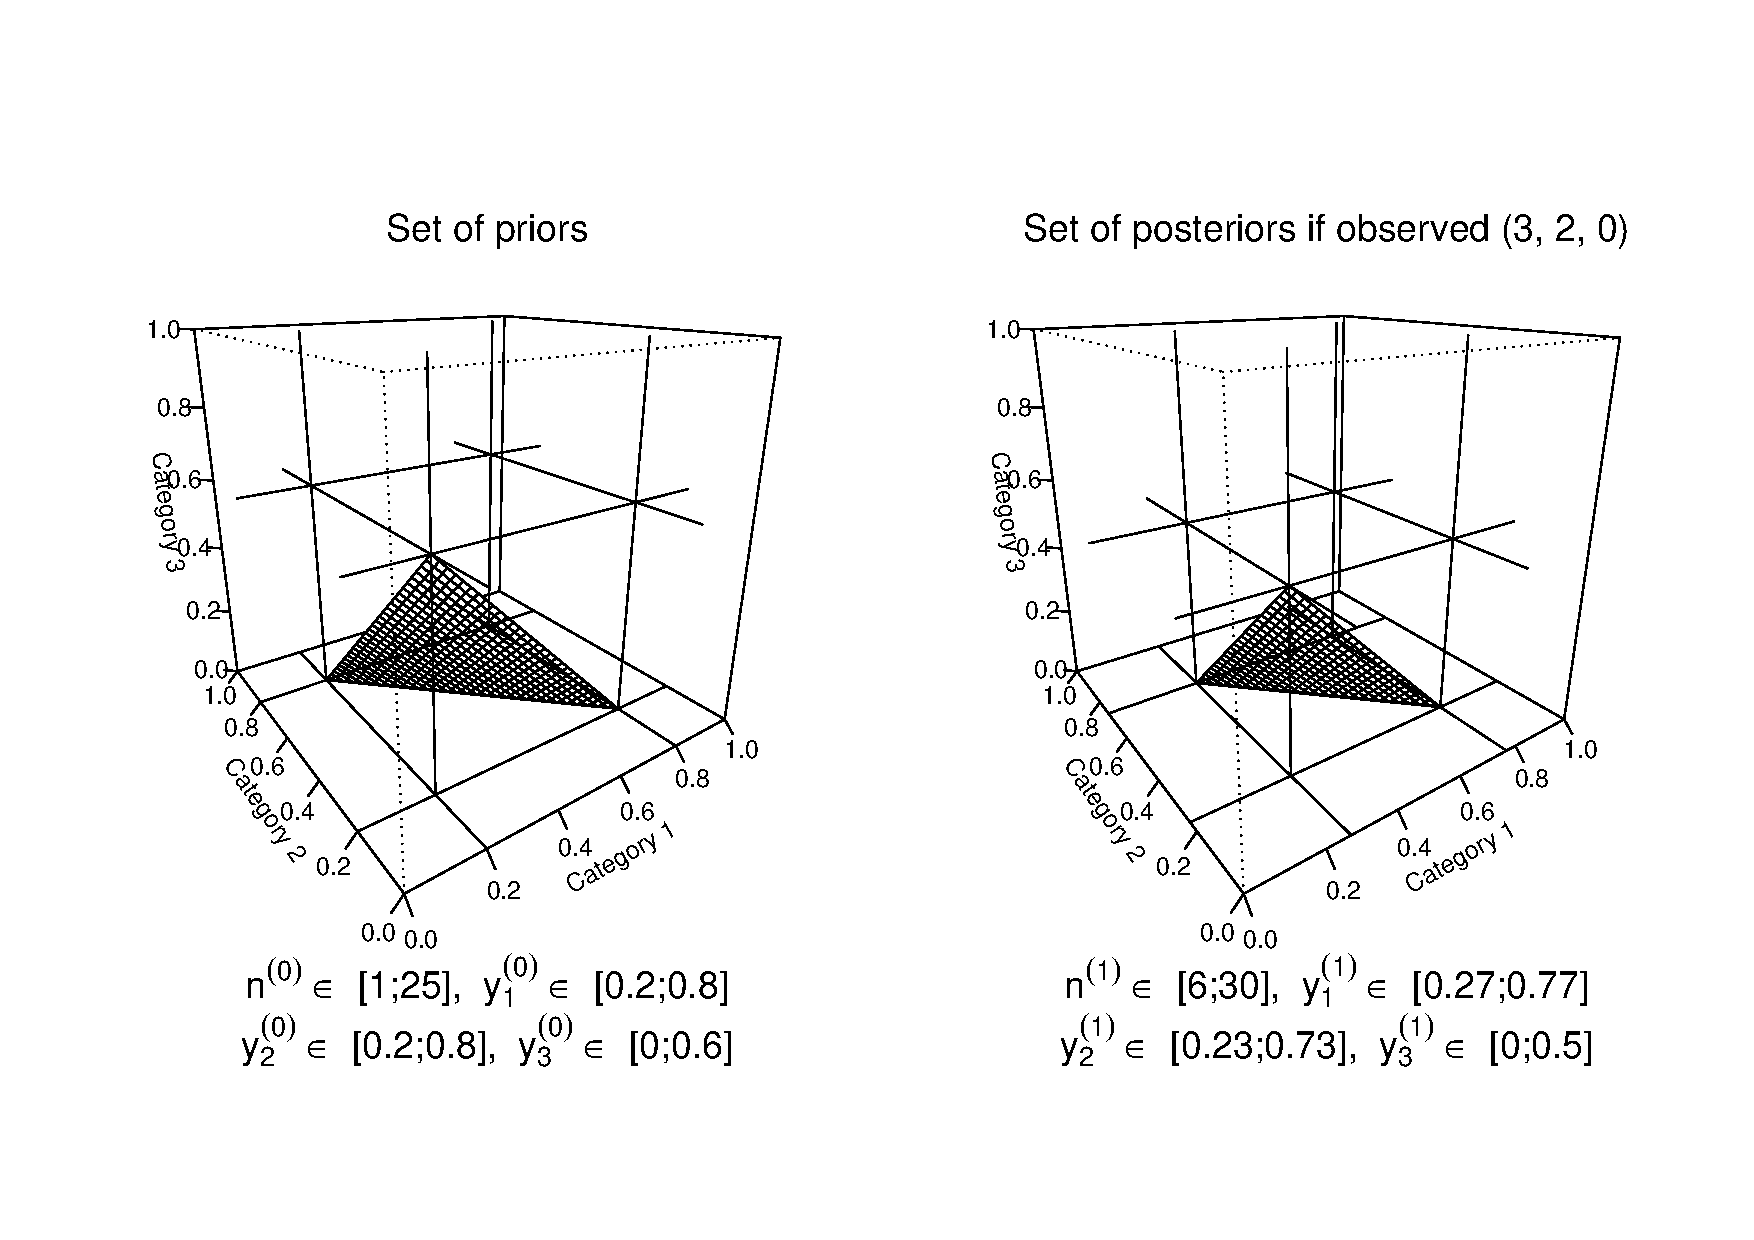
\includegraphics[trim = 150mm 25mm  20mm 20mm, clip, width=0.33\textwidth]{fig/jstp-paper_idm_nvar_zeile1-080331}%
\hspace*{-1.2ex}%
&%
\hspace*{-1.2ex}%
%\includegraphics[height=0.33\textwidth,angle=-90,bb = 100 470 520 790]{fig/jstp-paper_idm_nvar_zeile2-081205.ps}%
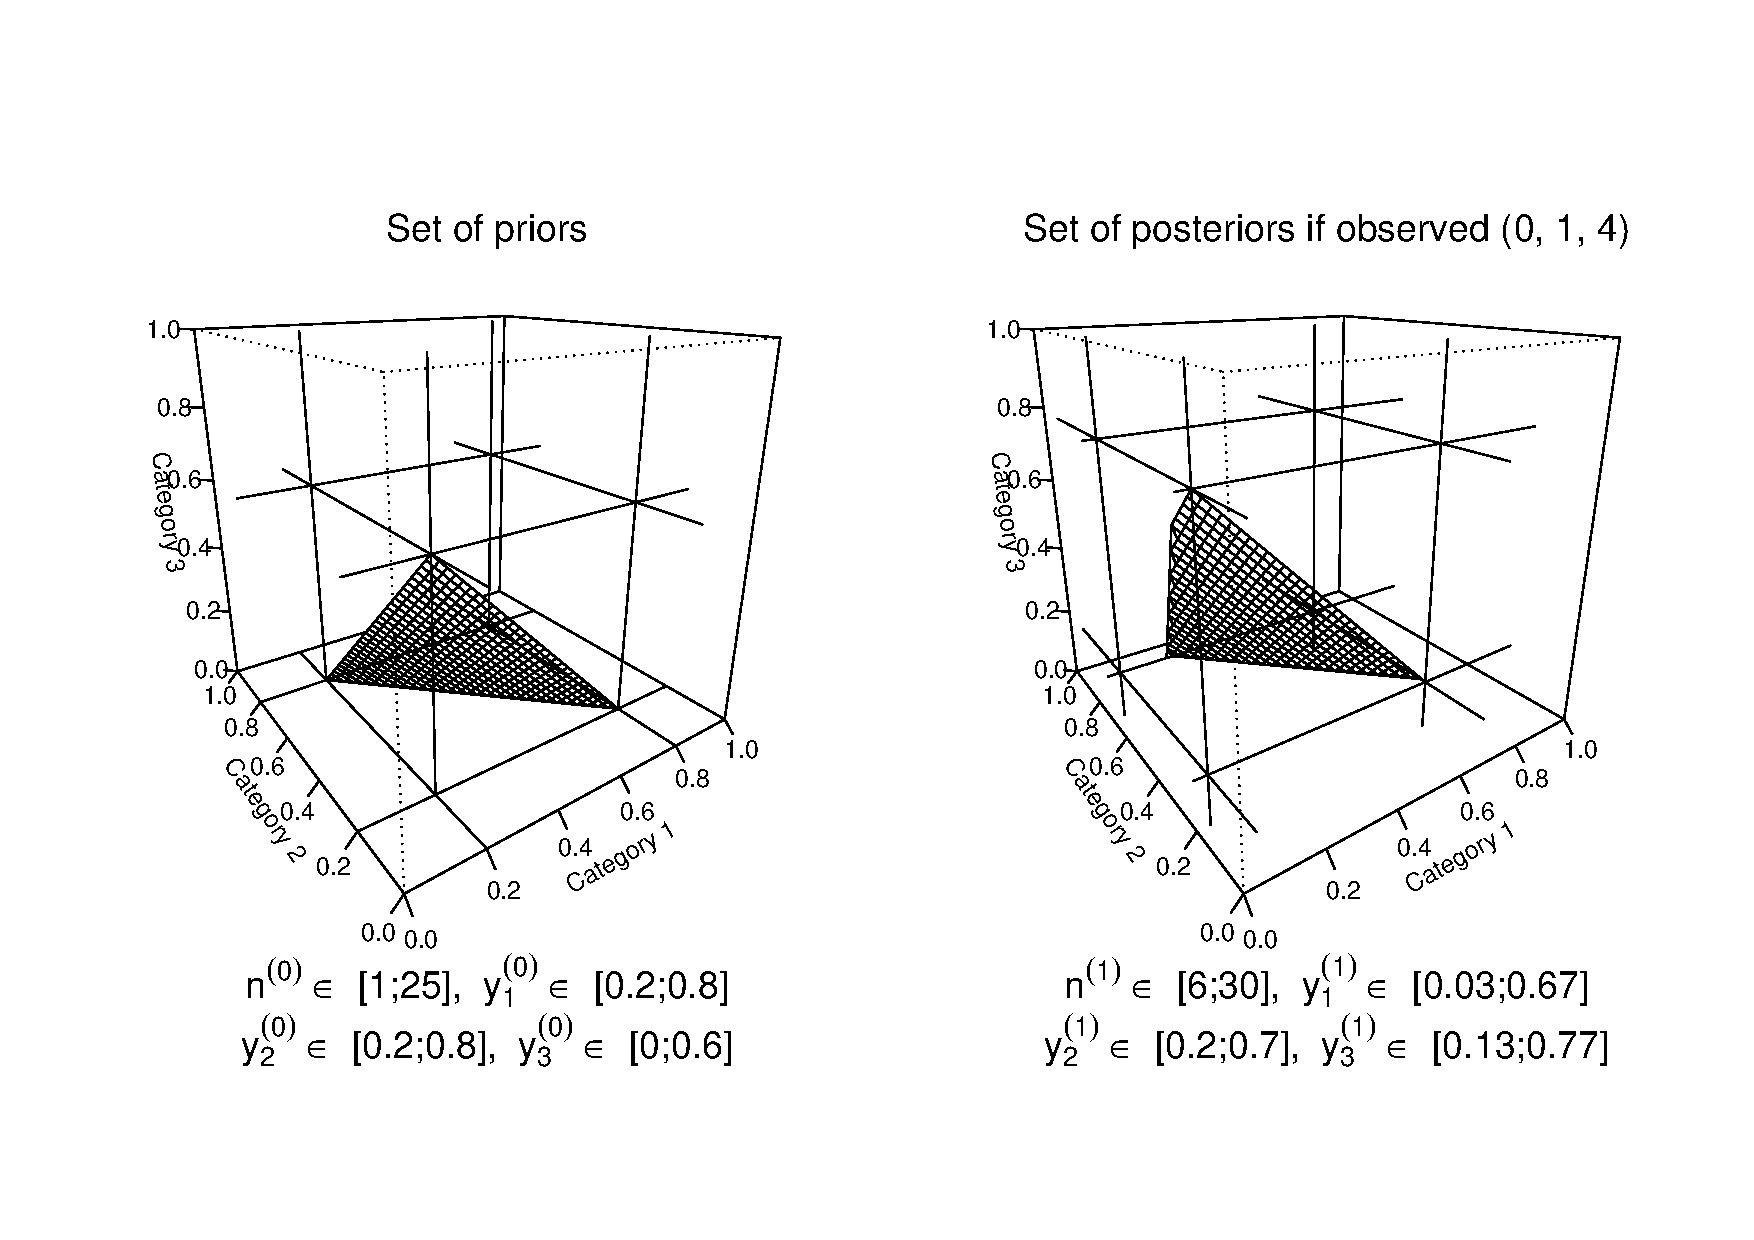
\includegraphics[trim = 150mm 25mm  20mm 20mm, clip, width=0.33\textwidth]{fig/jstp-paper_idm_nvar_zeile2-081205}%
\hspace*{-1.2ex}%
\end{tabular}%
\caption{
Prior (left) and posterior (center, right) credal sets for samples from
$\mult(\btheta)$ in accordance with (center) and contrary to (right)
prior beliefs. As in Figure~\ref{fig:nv-nvar-vertfu}, with \nymodel s
the sets differ in size according to the degree of prior-data conflict
induced by the observations.
}
\label{fig:idm-nvar-nopdc}
\end{figure}


\begin{example}[Dirichlet-Multinomial model, continued]
\label{ex:jstp-8}
For the Dirichlet-Multinomial model (Examples~\ref{ex:ymodel-idm} and \ref{ex:jstp-6}),
the behavior of the \nymodel\ is visualized in Figure~\ref{fig:idm-nvar-nopdc}. Here, the same set
of main parameters as in Figure~\ref{fig:idm-nfest-nopdc} is updated, leading
to plane cutouts (symbolizing posterior parameter sets) that
differ not only in location as before, but also in size (and shape) for the
two cases. For the center graph, prior assumptions on the category
probabilities are in accordance with the observations 3, 2 and 0
for category one, two, and three, respectively, and thus the
posterior plane cutout is a subset of the prior plane. In
contrast, when observations 0, 1, and 4 are made, being in
conflict with the prior assumptions for category one and three,
the resulting posterior parameter intervals for those two
categories do actually get wider, as can be seen in the right
graph, and thus, inference drawn in this case is more cautious.
\end{example}

\begin{figure} %trim = l b r t
%\includegraphics[height=0.99\textwidth,angle=-90,bb = 20 15 575 825]{fig/jstp-paper_nv_nvar_HPD_n-infty_081201.ps}%
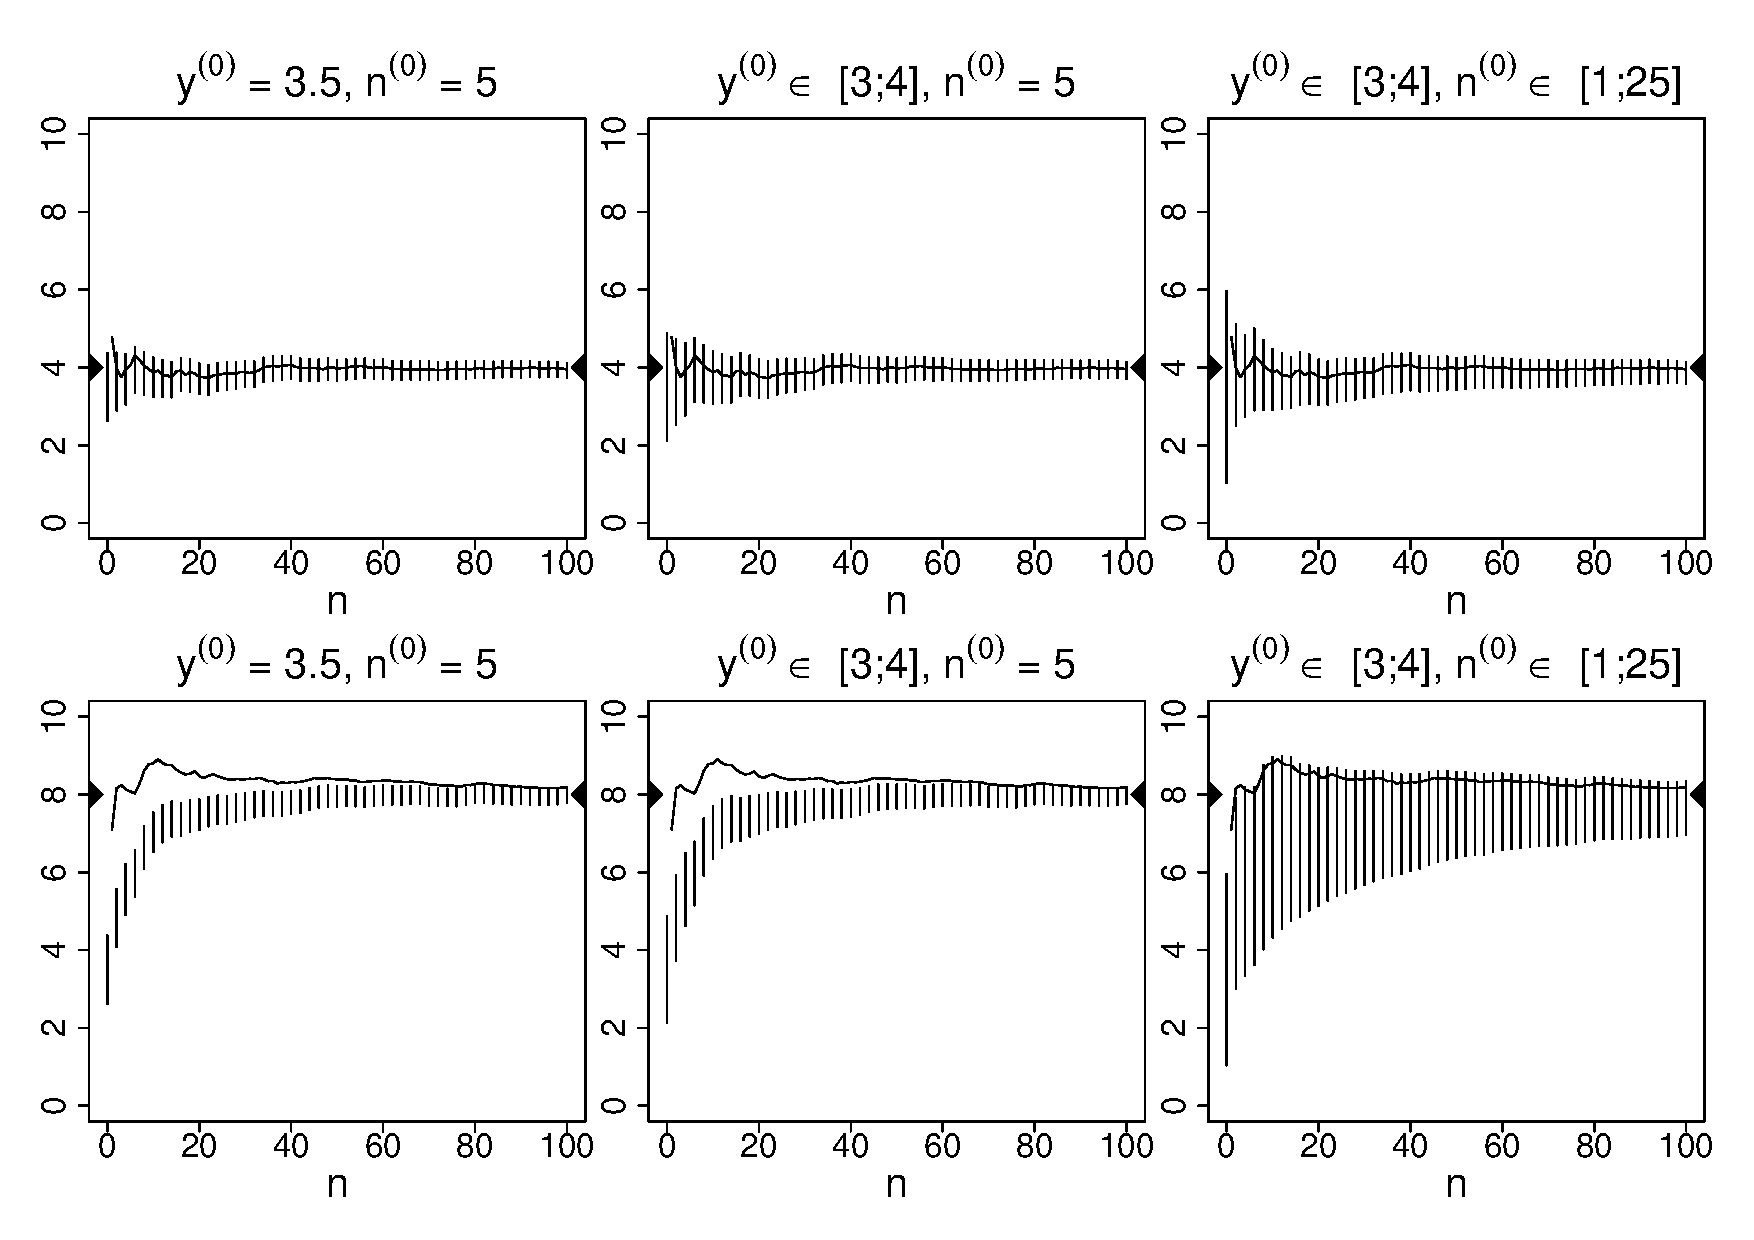
\includegraphics[trim = 5mm 5mm 5mm 5mm, clip, width=\textwidth]{fig/jstp-paper_nv_nvar_HPD_n-infty_081201}%
\caption{(Unions of) 95\%-posterior HD intervals (vertical lines) for
observations in accordance (upper row, drawn from $\mbox{N}(4,1)$)
and in conflict (lower row, drawn from $\mbox{N}(8,1)$) with prior assumptions
based on a single prior (left), an \ymodel\ (center) and a \nymodel\ (right)
in dependence on the sample size $n$. The development of the sample mean is
indicated by the wiggly line. Through the averaging, the HD intervals in the
lower left and center graph are not enlarged but only shifted and thus do not cover the sample mean.}
\label{fig:nv-nvar-kinfty}
\end{figure}

\begin{example}[Larger sample sizes]
\label{ex:jstp-9}
Still, sufficiently precise inference can be drawn when the sample
size gets much larger with respect to the prior strength, giving
data more weight than the prior guess. When no prior-data conflict
occurs, the imprecision obtained with \nymodel s is not
substantially larger than obtained with \ymodel s or even with a
classical, precise prior. These three model classes are compared by means
of the Normal-Normal model (Examples~\ref{ex:ymodel-nv}, \ref{ex:jstp-7} and \ref{ex:jstp-7})
in Figure~\ref{fig:nv-nvar-kinfty}, where the first
column gives posterior HD (further denoted by HPD) intervals for a
precise prior, the second column unions of HPD intervals for the
\ymodel, and the third column unions of HPD intervals for the
\nymodel, in all three cases drawn as vertical black lines for
sample sizes $n=2,4,6,\ldots,100$.

In the upper row, these prior models are updated successively with
observations drawn from a $\norm(4,1)$ being in accordance with the prior assumptions,
whereas for the lower row, observations in conflict with the prior
assumptions were simulated by observations drawn from a $\norm(8,1)$.
In the upper row, the (unions of)
intervals tend to the sample mean indicated by the wiggly line
more or less uniformly for all three models. Naturally, the most
precise prior gives the most precise posterior inferences, but the
HPD interval lengths do not differ excessively between the model classes, especially
when the sample size $n$ approaches $100$.

The lower row demonstrates the deficiency that the classical and
the \ymodel\ unfortunately share. For them, observations confronting
the prior assumptions lead only to an adjustment in location of
the intervals through the averaging, but not in their length, giving
a false certainty in posterior inference. Here, the \nymodel\ is
more truthful to the character of the situation, giving very wide
unions of HPD intervals for low sample sizes covering both the a priori
assumed range and the sample mean. With growing sample size, more
confidence is given to the data, and thus, the unions of HPD intervals
tend the more to the sample mean the larger the sample gets.
\end{example}


\subsection{Concluding remarks}
\label{sec:6-gw-071216}

***change it or leave it? draw links to other chapters and sections?***

In this ***paper*** we considered generalized Bayesian inference
in a wide class of imprecise probability models. We first
demonstrated that, in their originally proposed form, these models
do not react to prior-data conflict and so do not utilize
the full expressive power of imprecise probabilities. We
extended these models such that the natural relationship between
knowledge and imprecision is reestablished: the higher the
discrepancy between prior assumptions and sample observations the
more cautious the posterior inference. We compare the previous
modelling and our extension in two running examples covering two
widely used situations, inference from a scaled normal and
from a multinomial distribution, corroborating that our extension
shows promising behavior.

Further research will start with a more detailed study of
the behavior of the proposed model, also taking into consideration
that it may have some problems with dealing with very extreme
degrees of conflict. Then careful attention should also be paid to
other approaches for generalized Bayesian inference in exponential
families \parencite{1993:coolen, 1997:boratynska} under prior data
conflict, as well as to a thorough comparison of the inference
developed here with the discretization-based models considered by
\textcite{2005:whitcomb}, and with the approaches of \textcite{1991:pericchi}
and \textcite{1994:coolen}, who use different prior classes.

Far beyond these further developments, it should well be
remembered that this ***paper*** consciously confined the whole
argumentation to a certain Bayesian setting: we studied how far
one can go \emph{if} one relies strictly on the generalized Bayes
rule, transferring sets of priors to sets of posteriors element by
element via Bayes rule. Alternative learning
rules, including the approaches enumerated at Section~***paper intro*** %\ref{sec:intro},
could prove very important as, to use one of the referees'
felicitous words, ``Bayesian methods cannot allow for surprise, the same is
true for robustified or generalized Bayesian methods, although these
may hide this shortcoming better. One could argue, therefore, that
they cannot be used to represent learning.''

\subsection*{Acknowledgements}
We would like to thank two anonymous referees for their very stimulating comments.



%\clearpage


\section{***Software***}

seperate section, or integrate into jstp?

\section{***Isipta'07 paper***}

seperate section, or integrate into jstp?

